\documentclass[11pt, letterpaper]{article}

% Fonts and Encoding
\usepackage[utf8]{inputenc}
\usepackage[T1]{fontenc}
\usepackage{lmodern} % High-quality Latin Modern vector font

% Math and Symbols
\usepackage{amsmath, amssymb, amsthm, amsfonts, mathrsfs, mathtools}

% Layout and Geometry
\usepackage{geometry}
\geometry{letterpaper, margin=1in}
\setlength{\parindent}{0pt}
\setlength{\parskip}{0.6em}

% Formatting and Graphics
\usepackage{graphicx, xcolor, enumitem, booktabs, array, tabularx}

% TikZ for Illustrations
\usepackage{tikz}
\usetikzlibrary{arrows.meta, positioning, shapes.geometric, calc, backgrounds, matrix}

% Clickable Links and TOC
\usepackage{hyperref}
\hypersetup{
    colorlinks=true,
    linkcolor=blue,
    filecolor=magenta,      
    urlcolor=cyan,
    pdftitle={Inner Product Spaces (Section 6.7)},
}

% Theorem Environments
\newtheorem{theorem}{Theorem}[section]
\newtheorem{lemma}[theorem]{Lemma}
\newtheorem{proposition}[theorem]{Proposition}
\newtheorem{corollary}[theorem]{Corollary}
\theoremstyle{definition}
\newtheorem{definition}{Definition}[section]
\newtheorem{axiom}{Axiom}[section]
\newtheorem{example}{Example}[section]
\theoremstyle{remark}
\newtheorem{remark}{Remark}[section]

% Custom Commands (Enforced standard notation)
\newcommand{\R}{\mathbb{R}}
\newcommand{\N}{\mathbb{N}}
\newcommand{\Z}{\mathbb{Z}}
\newcommand{\Q}{\mathbb{Q}}
\newcommand{\E}{\mathbb{E}}
\newcommand{\Prob}{\mathbb{P}}
\newcommand{\F}{\mathcal{F}}

\title{Inner Product Spaces (Section 6.7):\\Practice Problem Sets and Detailed Solutions}
\author{Tashfeen Omran}
\date{\today}

\begin{document}

\maketitle
\tableofcontents
\newpage

\section{Concept Checklist and Question Mapping}

This mastery set covers every core concept, proof technique, algebraic shortcut, standard extension, and diagnostic pitfall in \textbf{Section 6.7: Inner Product Spaces}. Thirty-five original problems have been curated and weighted toward the structurally deeper concepts—Gram--Schmidt orthogonalization, orthogonal projection and best approximation, positive-definiteness (Axiom 4) verification for pullbacks and constrained forms, Cauchy--Schwarz inequality proofs, and advanced generalizations.

\subsection{Problem Types and General Approach}

\begin{description}
    \item[{Type 1: Weighted Inner Products on $\mathbb{R}^n$ (Problems 1--3, 13)}]
    \textbf{Assigned Problems:} 1, 2, 3, 13(b).\\
    \textbf{Strategic Workflow:} Identify the positive weights $c_1, \dots, c_n > 0$ in $\langle \mathbf{u}, \mathbf{v} \rangle = \sum_{i=1}^n c_i u_i v_i$. Compute $\|\mathbf{v}\|^2 = \langle \mathbf{v}, \mathbf{v} \rangle$ and take the nonnegative square root only at the final step. For orthogonality constraints, solve $\langle \mathbf{z}, \mathbf{y} \rangle = 0$ as a homogeneous linear equation; for parameter bounds guaranteeing Axiom 4, complete the square on $\langle \mathbf{u}, \mathbf{u} \rangle$.

    \item[{Type 2: Evaluation Inner Products on $\mathbb{P}_n$ (Problems 4--7, 13)}]
    \textbf{Assigned Problems:} 4, 5, 6, 7, 13(a).\\
    \textbf{Strategic Workflow:} Exploit the evaluation isomorphism $\mathbb{P}_n \cong \mathbb{R}^{n+1}$ by evaluating every polynomial at the $n+1$ distinct nodes $t_0, \dots, t_n$ first. Reduce inner products, norms, and orthogonal projections $\operatorname{proj}_W q = \sum_{i=1}^p \frac{\langle q, w_i \rangle}{\langle w_i, w_i \rangle} w_i$ to ordinary dot products of value vectors, reassembling the polynomial in $t$ only at the end. Verify that at least $n+1$ distinct nodes are present so Axiom 4 holds.

    \item[{Type 3: Discrete Gram--Schmidt Orthogonalization and Rescaling (Problems 8--10)}]
    \textbf{Assigned Problems:} 8, 9, 10.\\
    \textbf{Strategic Workflow:} Construct the orthogonal basis $\{p_0, \dots, p_k\}$ sequentially via $p_k = x_k - \sum_{j=0}^{k-1} \frac{\langle x_k, p_j \rangle}{\langle p_j, p_j \rangle} p_j$. On symmetric nodes around $0$, apply parity rules immediately to eliminate inner products between even and odd polynomials. On asymmetric nodes, work systematically with column value vectors. When target node values are specified, evaluate the raw orthogonal polynomial at the nodes and multiply by the reciprocal scalar factor.

    \item[{Type 4: Axiom Verification and Pullback Inner Products (Problems 11--14)}]
    \textbf{Assigned Problems:} 11, 12, 13, 14.\\
    \textbf{Strategic Workflow:} Verify Axioms 1--4 in sequence. Symmetry, additivity, and homogeneity follow directly from linearity of the map ($A$ or $T$), integration, or differentiation. Isolate Axiom 4 ($\langle \mathbf{u}, \mathbf{u} \rangle \ge 0$ and $\langle \mathbf{u}, \mathbf{u} \rangle = 0 \iff \mathbf{u} = \mathbf{0}$) by invoking invertibility of $A$, injectivity of $T$, $n+1$ distinct polynomial roots, or continuity of $[f(t)]^2$. For non-invertible matrices or insufficient nodes, exhibit an explicit nonzero counterexample with $\langle \mathbf{u}, \mathbf{u} \rangle = 0$.

    \item[{Type 5: Axiomatic Proofs, Identities, and Conceptual Diagnostics (Problems 15--19)}]
    \textbf{Assigned Problems:} 15, 16, 17, 18, 19.\\
    \textbf{Strategic Workflow:} Reason strictly from Axioms 1--4 without assuming coordinate or integral formulas. Use Axiom 1 (symmetry) to transfer linearity into the second slot. Expand squared norms via $\langle \mathbf{u} \pm \mathbf{v}, \mathbf{u} \pm \mathbf{v} \rangle = \|\mathbf{u}\|^2 \pm 2\langle \mathbf{u}, \mathbf{v} \rangle + \|\mathbf{v}\|^2$ to derive the Polarization Identity, Parallelogram Law, and Pythagorean Theorem. Test True/False claims against Axiom 4, bilinearity ($\langle c\mathbf{u}, c\mathbf{v} \rangle = c^2\langle \mathbf{u}, \mathbf{v} \rangle$), and orthogonality requirements.

    \item[{Type 6: Inequality Proofs via Cauchy--Schwarz and Triangle Inequalities (Problems 3, 20--22)}]
    \textbf{Assigned Problems:} 3, 20, 21, 22.\\
    \textbf{Strategic Workflow:} For numerical checks, compare $|\langle \mathbf{x}, \mathbf{y} \rangle|^2$ against $\|\mathbf{x}\|^2 \|\mathbf{y}\|^2$ to avoid nested radicals. For algebraic or integral inequalities, reverse-engineer vectors $\mathbf{u}, \mathbf{v} \in \mathbb{R}^n$ or functions $f, g \in C[a, b]$ (frequently using square roots) so that $\langle \mathbf{u}, \mathbf{v} \rangle$ yields the bounded term and $\|\mathbf{u}\|^2\|\mathbf{v}\|^2$ yields the bounding product. Derive the abstract Cauchy--Schwarz inequality from $\operatorname{proj}_{\operatorname{Span}\{\mathbf{u}\}} \mathbf{v}$ and deduce the Triangle Inequality by expanding $\|\mathbf{u}+\mathbf{v}\|^2$.

    \item[{Type 7: Integral Inner Products and Projections on {$C[a, b]$} (Problems 23--26)}]
    \textbf{Assigned Problems:} 23, 24, 25, 26.\\
    \textbf{Strategic Workflow:} Compute $\langle f, g \rangle = \int_a^b f(t)g(t)\,dt$ and $\|f\|^2 = \int_a^b [f(t)]^2\,dt$ carefully over the prescribed limits $[a, b]$. When projecting onto a subspace of polynomials (such as Legendre polynomials on $[-1, 1]$), confirm orthogonality of the basis first, use parity on $[-a, a]$, and apply the Best Approximation Theorem to find both $\hat{f}$ and the minimal $L^2$-error $\|f - \hat{f}\|$.

    \item[{Type 8: Continuous Gram--Schmidt on Polynomial and Trigonometric Spaces (Problems 27--29)}]
    \textbf{Assigned Problems:} 27, 28, 29.\\
    \textbf{Strategic Workflow:} Combine definite integration with parity and periodicity simplifications ($\int_{-a}^a (\text{odd})\,dt = 0$ and $\int_0^{2\pi} \cos^k t\,dt = \int_0^{2\pi} \sin^k t\,dt = 0$ for odd $k$). Use trigonometric power-reduction identities and multiple-angle identities ($\cos 2t$, $\sin 3t$), as well as integration by parts for mixed algebraic-trigonometric Fourier projections.

    \item[{Type 9: Advanced Extensions --- Hermitian, Weighted Integral, Frobenius, and Bessel (Problems 30--33)}]
    \textbf{Assigned Problems:} 30, 31, 32, 33.\\
    \textbf{Strategic Workflow:} Over $\mathbb{C}^n$, enforce conjugate symmetry $\langle \mathbf{u}, \mathbf{v} \rangle = \overline{\langle \mathbf{v}, \mathbf{u} \rangle}$ and conjugate linearity $\langle \mathbf{u}, c\mathbf{v} \rangle = \overline{c}\langle \mathbf{u}, \mathbf{v} \rangle$. For weighted integrals $\int_a^b f(t)g(t)w(t)\,dt$, incorporate $w(t)$ in every inner product and verify Axiom 4 via continuity when $w$ vanishes at an endpoint. On $M_{m\times n}(\mathbb{R})$, use $\langle A, B \rangle_F = \operatorname{tr}(A^T B)$ to project matrices onto symmetric and skew-symmetric subspaces. Apply the Pythagorean identity to orthogonal projections onto orthonormal sets to establish Bessel's Inequality and Parseval's Identity.

    \item[{Type 10: Diagnostic Flaw Analysis (Problems 34--35)}]
    \textbf{Assigned Problems:} 34, 35.\\
    \textbf{Strategic Workflow:} Audit each solution step-by-step for the classic traps of Section 6.7: dividing by $\|g\|$ instead of $\|g\|^2$ in projections, applying coordinate-wise projection formulas to non-orthogonal spanning sets, omitting the converse implication $\langle \mathbf{u}, \mathbf{u} \rangle = 0 \implies \mathbf{u} = \mathbf{0}$ for singular pullback matrices, and misapplying homogeneity as $\langle c\mathbf{u}, c\mathbf{u} \rangle = c\langle \mathbf{u}, \mathbf{u} \rangle$ instead of $c^2\langle \mathbf{u}, \mathbf{u} \rangle$.
\end{description}

\subsection{Master Concept Coverage Matrix}

\renewcommand{\arraystretch}{1.5}
\begin{tabularx}{\textwidth}{>{\bfseries}l X c}
\toprule
Problem Type & Core Concepts, Tricks, and Skills Tested & Problem Numbers \\
\midrule
Type 1 & Weighted inner products on $\mathbb{R}^n$, norms, distances, orthogonality, positive-definiteness parameter bounds & 1, 2, 3, 13(b) \\
Type 2 & Evaluation isomorphism $\mathbb{P}_n \cong \mathbb{R}^{n+1}$, norms, projections, best approximation error, minimum node count & 4, 5, 6, 7, 13(a) \\
Type 3 & Discrete Gram--Schmidt on symmetric and asymmetric nodes, parity shortcuts, basis rescaling to target values & 8, 9, 10 \\
Type 4 & Pullback inner products $\langle \mathbf{u}, \mathbf{v} \rangle = (A\mathbf{u})\cdot(A\mathbf{v})$ and $T(\mathbf{u})\cdot T(\mathbf{v})$, Sobolev-type inner product, singular counterexamples & 11, 12, 13, 14 \\
Type 5 & Axiomatic proofs from Axioms 1--4, bilinearity, Polarization Identity, Parallelogram Law, non-Euclidean norm test, T/F diagnostics & 15, 16, 17, 18, 19 \\
Type 6 & Cauchy--Schwarz numerical check, abstract proof via projection, Triangle Inequality, algebraic and integral inequalities & 3, 20, 21, 22 \\
Type 7 & Unweighted integral inner products on $C[a, b]$, orthogonality, Legendre projection, shifted Legendre Gram--Schmidt & 23, 24, 25, 26 \\
Type 8 & Cubic orthogonal polynomials on $[-a, a]$, trigonometric Gram--Schmidt, power-reduction/triple-angle formulas, Fourier projection & 27, 28, 29 \\
Type 9 & Hermitian inner products on $\mathbb{C}^n$, weighted integral inner products, Frobenius matrix inner product, Bessel's Inequality & 30, 31, 32, 33 \\
Type 10 & Detecting projection denominator errors, non-orthogonal basis errors, incomplete Axiom 4 checks, and scalar homogeneity traps & 34, 35 \\
\bottomrule
\end{tabularx}

\newpage

\section{Problem Sets}

\subsection{Weighted Inner Products on Euclidean Spaces (Problems 1--3)}

\textbf{Problem 1.} Let $\mathbb{R}^2$ have the weighted inner product $\langle \mathbf{u}, \mathbf{v} \rangle = 3u_1v_1 + 7u_2v_2$, and let $\mathbf{x} = (2, -1)$ and $\mathbf{y} = (7, 3)$.
\begin{enumerate}[label=(\alph*)]
    \item Compute $\|\mathbf{x}\|$, $\|\mathbf{y}\|$, $|\langle \mathbf{x}, \mathbf{y} \rangle|^2$, and $\operatorname{dist}(\mathbf{x}, \mathbf{y})$.
    \item Describe all vectors $\mathbf{z} = (z_1, z_2) \in \mathbb{R}^2$ that are orthogonal to $\mathbf{y}$.
\end{enumerate}

\textbf{Problem 2.} Let $\mathbb{R}^3$ have the weighted inner product $\langle \mathbf{u}, \mathbf{v} \rangle = 2u_1v_1 + 5u_2v_2 + u_3v_3$. Let $\mathbf{x} = (1, 2, -2)$ and $\mathbf{w} = (2, -1, k)$, where $k \in \mathbb{R}$.
\begin{enumerate}[label=(\alph*)]
    \item Find a unit vector $\mathbf{u} \in \mathbb{R}^3$ in the direction of $\mathbf{x}$.
    \item Determine the value of $k$ for which $\mathbf{x}$ and $\mathbf{w}$ are orthogonal.
    \item For $k = 1$, compute $\operatorname{proj}_{\operatorname{Span}\{\mathbf{x}\}} \mathbf{w}$.
\end{enumerate}

\textbf{Problem 3.} Let $\mathbb{R}^2$ have the weighted inner product $\langle \mathbf{u}, \mathbf{v} \rangle = 6u_1v_1 + 2u_2v_2$. Verify that the Cauchy--Schwarz inequality holds for $\mathbf{x} = (2, -5)$ and $\mathbf{y} = (-3, 4)$, and determine whether equality holds.

\subsection{Evaluation Inner Products on Polynomial Spaces (Problems 4--7)}

\textbf{Problem 4.} Let $\mathbb{P}_2$ have the inner product given by evaluation at $-2, 0, 2$:
\[
\langle p, q \rangle = p(-2)q(-2) + p(0)q(0) + p(2)q(2).
\]
Compute $\langle p, q \rangle$, $\|p\|$, and $\|q\|$ for $p(t) = 3 - t$ and $q(t) = 2t^2 - 1$.

\textbf{Problem 5.} Let $\mathbb{P}_2$ have the inner product given by evaluation at $-1, 1, 3$:
\[
\langle p, q \rangle = p(-1)q(-1) + p(1)q(1) + p(3)q(3).
\]
For $p(t) = 1 + 2t - t^2$ and $q(t) = 4 - t^2$, compute $\langle p, q \rangle$, $\|p\|$, $\|q\|$, and $\operatorname{proj}_{\operatorname{Span}\{p\}} q$.

\textbf{Problem 6.} Using the space $\mathbb{P}_2$ and polynomials $p(t) = 3 - t$ and $q(t) = 2t^2 - 1$ from Problem 4, compute $\hat{q} = \operatorname{proj}_{\operatorname{Span}\{p\}} q$ and find the minimum distance $\operatorname{dist}(q, \operatorname{Span}\{p\}) = \|q - \hat{q}\|$.

\textbf{Problem 7.} Let $\mathbb{P}_3$ have the inner product given by evaluation at $-3, -1, 1, 3$. Using the orthogonal set $\{p_0, p_1, p_2\}$ given by $p_0(t) = 1$, $p_1(t) = t$, and $p_2(t) = t^2 - 5$, find the best approximation to $p(t) = 2t^3 - t^2 + 3$ by polynomials in $W = \operatorname{Span}\{p_0, p_1, p_2\}$.

\subsection{Discrete Gram--Schmidt and Basis Rescaling (Problems 8--10)}

\textbf{Problem 8.} Let $\mathbb{P}_3$ have the inner product given by evaluation at $-2, -1, 1, 2$. Let $x_0(t) = 1$, $x_1(t) = t$, and $x_2(t) = t^2$.
\begin{enumerate}[label=(\alph*)]
    \item Compute the orthogonal projection of $x_2$ onto $\operatorname{Span}\{x_0, x_1\}$.
    \item Find a polynomial $q$ orthogonal to $x_0$ and $x_1$ such that $\{x_0, x_1, q\}$ is an orthogonal basis for $\operatorname{Span}\{1, t, t^2\}$. Scale $q$ so that its vector of values at $(-2, -1, 1, 2)$ is $(1, -1, -1, 1)^T$.
\end{enumerate}

\textbf{Problem 9.} Let $\mathbb{P}_4$ have the inner product given by evaluation at $-3, -1, 0, 1, 3$, and let $p_0(t) = 1$, $p_1(t) = t$, and $p_2(t) = t^2 - 4$.
\begin{enumerate}[label=(\alph*)]
    \item Verify that $\{p_0, p_1, p_2\}$ is an orthogonal set in $\mathbb{P}_4$.
    \item Compute the orthogonal projection of $t^3$ onto $\operatorname{Span}\{p_0, p_1, p_2\}$.
    \item Find the monic polynomial $p_3(t)$ such that $\{p_0, p_1, p_2, p_3\}$ is an orthogonal basis for $\mathbb{P}_3 \subset \mathbb{P}_4$, and also find the scalar multiple $\tilde{p}_3(t)$ whose vector of values at $(-3, -1, 0, 1, 3)$ is $(-1, 3, 0, -3, 1)^T$.
\end{enumerate}

\textbf{Problem 10.} Let $\mathbb{P}_3$ have the inner product given by evaluation at the asymmetric nodes $0, 1, 2, 3$:
\[
\langle p, q \rangle = p(0)q(0) + p(1)q(1) + p(2)q(2) + p(3)q(3).
\]
Apply the Gram--Schmidt process to $\{1, t, t^2\}$ to construct an orthogonal basis $\{p_0, p_1, p_2\}$ for $\mathbb{P}_2 \subset \mathbb{P}_3$.

\subsection{Axiom Verification and Pullback Inner Products (Problems 11--14)}

\textbf{Problem 11.} Let $A$ be an $n \times n$ real matrix and define $\langle \mathbf{u}, \mathbf{v} \rangle = (A\mathbf{u}) \cdot (A\mathbf{v}) = (A\mathbf{u})^T(A\mathbf{v})$ for $\mathbf{u}, \mathbf{v} \in \mathbb{R}^n$.
\begin{enumerate}[label=(\alph*)]
    \item Prove that if $A$ is invertible, then $\langle \cdot, \cdot \rangle$ defines an inner product on $\mathbb{R}^n$.
    \item Let $A = \begin{bmatrix} 3 & -6 \\ -1 & 2 \end{bmatrix}$. Does $\langle \mathbf{u}, \mathbf{v} \rangle = (A\mathbf{u}) \cdot (A\mathbf{v})$ define an inner product on $\mathbb{R}^2$? Justify your answer.
\end{enumerate}

\textbf{Problem 12.} Let $T : V \to \mathbb{R}^n$ be a one-to-one linear transformation from a real vector space $V$ into $\mathbb{R}^n$.
\begin{enumerate}[label=(\alph*)]
    \item Prove that $\langle \mathbf{u}, \mathbf{v} \rangle = T(\mathbf{u}) \cdot T(\mathbf{v})$ defines an inner product on $V$.
    \item Define $T : \mathbb{P}_2 \to \mathbb{R}^3$ by $T(p) = (p(0), p'(0), p''(0))^T$. Verify that $T$ is linear and one-to-one, and use the induced inner product $\langle p, q \rangle = T(p) \cdot T(q)$ to compute $\langle p, q \rangle$ for $p(t) = 2 - 3t + 4t^2$ and $q(t) = 5 + t - \frac{1}{2}t^2$.
\end{enumerate}

\textbf{Problem 13.}
\begin{enumerate}[label=(\alph*)]
    \item Explain why the formula $\langle p, q \rangle = p(-1)q(-1) + p(0)q(0) + p(1)q(1)$ does \emph{not} define an inner product on $\mathbb{P}_3$ by exhibiting an explicit nonzero polynomial $p \in \mathbb{P}_3$ with $\langle p, p \rangle = 0$.
    \item Find all real numbers $k \in \mathbb{R}$ for which $\langle \mathbf{u}, \mathbf{v} \rangle = 2u_1v_1 + ku_1v_2 + ku_2v_1 + 5u_2v_2$ defines an inner product on $\mathbb{R}^2$.
\end{enumerate}

\textbf{Problem 14.} Show that for $p, q \in \mathbb{P}_2$, the Sobolev-type formula
\[
\langle p, q \rangle = p(0)q(0) + \int_0^1 p'(t)q'(t)\,dt
\]
defines an inner product on $\mathbb{P}_2$.

\subsection{Axiomatic Proofs, Identities, and Conceptual Diagnostics (Problems 15--19)}

\textbf{Problem 15.} Let $V$ be a real inner product space. Using only the four defining axioms of an inner product, prove the following properties for all $\mathbf{u}, \mathbf{v}, \mathbf{w} \in V$ and all $a, b, c, d \in \mathbb{R}$:
\begin{enumerate}[label=(\alph*)]
    \item $\langle \mathbf{v}, \mathbf{0} \rangle = \langle \mathbf{0}, \mathbf{v} \rangle = 0$.
    \item $\langle \mathbf{u}, a\mathbf{v} + b\mathbf{w} \rangle = a\langle \mathbf{u}, \mathbf{v} \rangle + b\langle \mathbf{u}, \mathbf{w} \rangle$.
    \item $\langle c\mathbf{u}, d\mathbf{v} \rangle = cd\langle \mathbf{u}, \mathbf{v} \rangle$.
\end{enumerate}

\textbf{Problem 16.} Let $V$ be a real inner product space.
\begin{enumerate}[label=(\alph*)]
    \item If $\{\mathbf{u}, \mathbf{v}\}$ is an orthonormal set in $V$, compute $\|\mathbf{u} - \mathbf{v}\|$ and $\|3\mathbf{u} + 4\mathbf{v}\|$.
    \item If $\mathbf{u}$ and $\mathbf{v}$ are unit vectors in $V$ satisfying $\langle \mathbf{u}, \mathbf{v} \rangle = -\frac{1}{4}$, compute $\|2\mathbf{u} + 4\mathbf{v}\|$.
\end{enumerate}

\textbf{Problem 17.} Let $V$ be a real inner product space and let $\mathbf{u}, \mathbf{v} \in V$.
\begin{enumerate}[label=(\alph*)]
    \item Verify the Polarization Identity: $\langle \mathbf{u}, \mathbf{v} \rangle = \frac{1}{4}\|\mathbf{u} + \mathbf{v}\|^2 - \frac{1}{4}\|\mathbf{u} - \mathbf{v}\|^2$.
    \item Verify the Parallelogram Law: $\|\mathbf{u} + \mathbf{v}\|^2 + \|\mathbf{u} - \mathbf{v}\|^2 = 2\|\mathbf{u}\|^2 + 2\|\mathbf{v}\|^2$.
    \item Use part (b) to prove that the norm $\|\mathbf{x}\|_\infty = \max\{|x_1|, |x_2|\}$ on $\mathbb{R}^2$ cannot be induced by any inner product on $\mathbb{R}^2$.
\end{enumerate}

\textbf{Problem 18.} Let $V$ be a real inner product space.
\begin{enumerate}[label=(\alph*)]
    \item Prove the abstract Pythagorean Theorem: if $\langle \mathbf{u}, \mathbf{v} \rangle = 0$, then $\|\mathbf{u} + \mathbf{v}\|^2 = \|\mathbf{u}\|^2 + \|\mathbf{v}\|^2$.
    \item Let $W \subseteq V$ be a finite-dimensional subspace with orthogonal basis $\{\mathbf{w}_1, \dots, \mathbf{w}_p\}$, and define $\hat{\mathbf{v}} = \operatorname{proj}_W \mathbf{v} = \sum_{i=1}^p \frac{\langle \mathbf{v}, \mathbf{w}_i \rangle}{\langle \mathbf{w}_i, \mathbf{w}_i \rangle}\mathbf{w}_i$. Prove directly from the inner product axioms that $\mathbf{v} - \hat{\mathbf{v}}$ is orthogonal to every $\mathbf{w} \in W$, and deduce that $\|\mathbf{v}\|^2 = \|\hat{\mathbf{v}}\|^2 + \|\mathbf{v} - \hat{\mathbf{v}}\|^2$.
\end{enumerate}

\textbf{Problem 19.} Determine whether each statement is True or False in an arbitrary real inner product space $V$. Justify each True statement using axioms or theorems, and give an explicit counterexample for each False statement.
\begin{enumerate}[label=(\alph*)]
    \item If $\langle \mathbf{u}, \mathbf{u} \rangle = 0$, then $\mathbf{u} = \mathbf{0}$.
    \item If $\langle \mathbf{u}, \mathbf{v} \rangle = 0$, then either $\mathbf{u} = \mathbf{0}$ or $\mathbf{v} = \mathbf{0}$.
    \item $\langle c\mathbf{u}, c\mathbf{v} \rangle = c\langle \mathbf{u}, \mathbf{v} \rangle$ for all $\mathbf{u}, \mathbf{v} \in V$ and $c \in \mathbb{R}$.
    \item $\|\mathbf{u} + \mathbf{v}\| = \|\mathbf{u}\| + \|\mathbf{v}\|$ for all $\mathbf{u}, \mathbf{v} \in V$.
    \item If $|\langle \mathbf{u}, \mathbf{v} \rangle| = \|\mathbf{u}\|\|\mathbf{v}\|$ and $\mathbf{u} \neq \mathbf{0}$, then $\mathbf{v}$ is a scalar multiple of $\mathbf{u}$.
    \item For any basis $\{\mathbf{w}_1, \mathbf{w}_2\}$ of a $2$-dimensional subspace $W \subseteq V$, $\operatorname{proj}_W \mathbf{v} = \frac{\langle \mathbf{v}, \mathbf{w}_1 \rangle}{\langle \mathbf{w}_1, \mathbf{w}_1 \rangle}\mathbf{w}_1 + \frac{\langle \mathbf{v}, \mathbf{w}_2 \rangle}{\langle \mathbf{w}_2, \mathbf{w}_2 \rangle}\mathbf{w}_2$.
\end{enumerate}

\subsection{Cauchy--Schwarz and Triangle Inequality Proofs (Problems 20--22)}

\textbf{Problem 20.} Use the Cauchy--Schwarz inequality in $\mathbb{R}^3$ (with the standard dot product) by choosing strategic vectors $\mathbf{u}, \mathbf{v} \in \mathbb{R}^3$ to prove each inequality:
\begin{enumerate}[label=(\alph*)]
    \item For all $a, b, c \in \mathbb{R}$, $(a + b + c)^2 \le 3(a^2 + b^2 + c^2)$.
    \item For all $x, y, z > 0$, $(x + y + z)\left(\frac{1}{x} + \frac{1}{y} + \frac{1}{z}\right) \ge 9$.
\end{enumerate}

\textbf{Problem 21.} Let $V$ be any real inner product space and let $\mathbf{u}, \mathbf{v} \in V$.
\begin{enumerate}[label=(\alph*)]
    \item Prove the Cauchy--Schwarz inequality: $|\langle \mathbf{u}, \mathbf{v} \rangle| \le \|\mathbf{u}\|\|\mathbf{v}\|$.
    \item Use part (a) to prove the Triangle Inequality: $\|\mathbf{u} + \mathbf{v}\| \le \|\mathbf{u}\| + \|\mathbf{v}\|$.
\end{enumerate}

\textbf{Problem 22.} Let $V = C[a, b]$ have the inner product $\langle f, g \rangle = \int_a^b f(t)g(t)\,dt$, and suppose $h \in C[a, b]$ satisfies $h(t) > 0$ for all $t \in [a, b]$.
\begin{enumerate}[label=(\alph*)]
    \item Use the Cauchy--Schwarz inequality in $C[a, b]$ to prove that
    \[
    \left(\int_a^b h(t)\,dt\right)\left(\int_a^b \frac{1}{h(t)}\,dt\right) \ge (b - a)^2.
    \]
    \item Verify this inequality explicitly for $h(t) = e^t$ on $[0, 1]$, and determine whether equality holds.
\end{enumerate}

\subsection{Integral Inner Products and Projections on Function Spaces (Problems 23--26)}

\textbf{Problem 23.} Let $V = C[0, 1]$ have the inner product $\langle f, g \rangle = \int_0^1 f(t)g(t)\,dt$. Let $f(t) = 2 - 6t$ and $g(t) = 3t^2 - 2t$.
\begin{enumerate}[label=(\alph*)]
    \item Compute $\langle f, g \rangle$ and determine whether $f$ and $g$ are orthogonal.
    \item Compute $\|f\|$ and $\|g\|$.
\end{enumerate}

\textbf{Problem 24.} Let $V = C[0, 1]$ have the inner product $\langle f, g \rangle = \int_0^1 f(t)g(t)\,dt$. Let $f(t) = t^2$ and $g(t) = 1 + 2t$. Compute $\langle f, g \rangle$, $\|g\|$, and $\operatorname{proj}_{\operatorname{Span}\{g\}} f$.

\textbf{Problem 25.} Let $V = C[-1, 1]$ have the inner product $\langle f, g \rangle = \int_{-1}^1 f(t)g(t)\,dt$. Using the orthogonal Legendre basis $\left\{1, t, t^2 - \frac{1}{3}\right\}$ for $\mathbb{P}_2$, find the best approximation $\hat{f} \in \mathbb{P}_2$ to $f(t) = 5t^3 + 3t^2 - 1$, and compute the minimum $L^2$-error $\|f - \hat{f}\|$.

\textbf{Problem 26.} Let $V = C[0, 1]$ have the inner product $\langle f, g \rangle = \int_0^1 f(t)g(t)\,dt$. Apply the Gram--Schmidt process to $\{1, t, t^2\}$ to construct an orthogonal basis $\{p_0, p_1, p_2\}$ for $\mathbb{P}_2 \subset C[0, 1]$ (the shifted Legendre polynomials).

\subsection{Continuous Gram--Schmidt on Polynomial and Trigonometric Spaces (Problems 27--29)}

\textbf{Problem 27.} Let $V = C[-3, 3]$ have the inner product $\langle f, g \rangle = \int_{-3}^3 f(t)g(t)\,dt$. Apply the Gram--Schmidt process to $\{1, t, t^2, t^3\}$ to construct an orthogonal basis $\{p_0, p_1, p_2, p_3\}$ for $\mathbb{P}_3 \subset C[-3, 3]$.

\textbf{Problem 28.} Let $V = C[0, 2\pi]$ have the inner product $\langle f, g \rangle = \int_0^{2\pi} f(t)g(t)\,dt$. Apply the Gram--Schmidt process to $\{1, \sin t, \sin^2 t, \sin^3 t\}$ to construct an orthogonal basis $\{q_0, q_1, q_2, q_3\}$ for the subspace spanned by these four functions, and express $q_2$ and $q_3$ in terms of $\cos 2t$ and $\sin 3t$.

\textbf{Problem 29.} Let $V = C[-\pi, \pi]$ have the inner product $\langle f, g \rangle = \int_{-\pi}^{\pi} f(t)g(t)\,dt$.
\begin{enumerate}[label=(\alph*)]
    \item Verify that $\{1, \cos t, \sin t\}$ is an orthogonal set in $V$ and compute the squared norm of each function.
    \item Find the best approximation $\hat{f}$ to $f(t) = t^2 + t$ in $W = \operatorname{Span}\{1, \cos t, \sin t\}$.
\end{enumerate}

\subsection{Advanced Extensions: Hermitian, Weighted, Frobenius, and Bessel (Problems 30--33)}

\textbf{Problem 30.} In $\mathbb{C}^2$ equipped with the standard Hermitian inner product $\langle \mathbf{u}, \mathbf{v} \rangle = u_1\overline{v_1} + u_2\overline{v_2}$, let $\mathbf{u} = (2 - i, 1 + 3i)^T$, $\mathbf{v} = (1 + i, 2i)^T$, and $c = 1 - 2i$.
\begin{enumerate}[label=(\alph*)]
    \item Compute $\langle \mathbf{u}, \mathbf{v} \rangle$ and $\langle \mathbf{v}, \mathbf{u} \rangle$, and verify conjugate symmetry $\langle \mathbf{u}, \mathbf{v} \rangle = \overline{\langle \mathbf{v}, \mathbf{u} \rangle}$.
    \item Compute $\|\mathbf{u}\|$ and $\|\mathbf{v}\|$.
    \item Verify conjugate linearity in the second slot by computing both $\langle \mathbf{u}, c\mathbf{v} \rangle$ and $\overline{c}\langle \mathbf{u}, \mathbf{v} \rangle$.
\end{enumerate}

\textbf{Problem 31.} Let $V = C[0, 1]$ be equipped with the weighted integral inner product
\[
\langle f, g \rangle_w = \int_0^1 f(t)g(t)t^2\,dt,
\]
corresponding to the weight function $w(t) = t^2$.
\begin{enumerate}[label=(\alph*)]
    \item Explain carefully why Axiom 4 (positive-definiteness) holds on $C[0, 1]$ even though $w(0) = 0$.
    \item Apply the Gram--Schmidt process to $\{1, t, t^2\}$ to obtain an orthogonal basis $\{p_0, p_1, p_2\}$ for $\mathbb{P}_2$ under $\langle \cdot, \cdot \rangle_w$.
\end{enumerate}

\textbf{Problem 32.} Let $V = M_{2\times 2}(\mathbb{R})$ have the Frobenius inner product $\langle A, B \rangle_F = \operatorname{tr}(A^T B) = \sum_{i=1}^2 \sum_{j=1}^2 a_{ij}b_{ij}$. Let $W \subset V$ be the $3$-dimensional subspace of symmetric $2 \times 2$ matrices with orthogonal basis
\[
E_1 = \begin{bmatrix} 1 & 0 \\ 0 & 0 \end{bmatrix}, \qquad E_2 = \begin{bmatrix} 0 & 0 \\ 0 & 1 \end{bmatrix}, \qquad E_3 = \begin{bmatrix} 0 & 1 \\ 1 & 0 \end{bmatrix}.
\]
For $A = \begin{bmatrix} 2 & 5 \\ -1 & 4 \end{bmatrix}$:
\begin{enumerate}[label=(\alph*)]
    \item Compute $\hat{A} = \operatorname{proj}_W A$ and verify that $\hat{A} = \frac{1}{2}(A + A^T)$.
    \item Find $A_\perp = A - \hat{A}$, verify that $\langle \hat{A}, A_\perp \rangle_F = 0$, and verify the Pythagorean identity $\|A\|_F^2 = \|\hat{A}\|_F^2 + \|A_\perp\|_F^2$.
\end{enumerate}

\textbf{Problem 33.} Let $V$ be a real inner product space and let $\{\mathbf{e}_1, \dots, \mathbf{e}_k\}$ be an orthonormal set in $V$.
\begin{enumerate}[label=(\alph*)]
    \item Prove Bessel's Inequality: $\sum_{j=1}^k |\langle \mathbf{v}, \mathbf{e}_j \rangle|^2 \le \|\mathbf{v}\|^2$ for all $\mathbf{v} \in V$, and show that equality (Parseval's Identity) holds if and only if $\mathbf{v} \in \operatorname{Span}\{\mathbf{e}_1, \dots, \mathbf{e}_k\}$.
    \item Verify Bessel's Inequality for $f(t) = t^2$ in $C[-1, 1]$ using the two orthonormal Legendre functions $e_0(t) = \frac{1}{\sqrt{2}}$ and $e_1(t) = \sqrt{\frac{3}{2}}\,t$, and explain why equality does not hold.
\end{enumerate}

\subsection{Diagnostic Flaw Analysis (Problems 34--35)}

\textbf{Problem 34.} Each student solution below contains a single critical mathematical flaw. Identify the exact flawed step, explain in one or two sentences why it is invalid, and provide the corrected solution.
\begin{enumerate}[label=(\alph*)]
    \item \emph{Student A's Solution:} On $V = C[0, 1]$ with $\langle f, g \rangle = \int_0^1 f(t)g(t)\,dt$, find $\operatorname{proj}_W f$ for $f(t) = t^3$ and $W = \operatorname{Span}\{g\}$ with $g(t) = 3t$.
    \begin{enumerate}[label=Step \arabic*:]
        \item $\langle f, g \rangle = \int_0^1 3t^4\,dt = \frac{3}{5}$.
        \item $\|g\|^2 = \int_0^1 9t^2\,dt = 3$, so $\|g\| = \sqrt{3}$.
        \item $\operatorname{proj}_W f = \frac{\langle f, g \rangle}{\|g\|} g = \frac{3/5}{\sqrt{3}}(3t) = \frac{3\sqrt{3}}{5}t$.
    \end{enumerate}
    \item \emph{Student B's Solution:} On $V = \mathbb{P}_2$ with evaluation at $-1, 0, 1$, find $\operatorname{proj}_W q$ for $q(t) = t^2$ and $W = \operatorname{Span}\{p_1, p_2\}$ with $p_1(t) = 1$ and $p_2(t) = 1 + 2t$.
    \begin{enumerate}[label=Step \arabic*:]
        \item List value vectors at $(-1, 0, 1)$: $p_1 \leftrightarrow (1, 1, 1)^T$, $p_2 \leftrightarrow (-1, 1, 3)^T$, $q \leftrightarrow (1, 0, 1)^T$.
        \item $\langle q, p_1 \rangle = 2$, $\|p_1\|^2 = 3$; $\langle q, p_2 \rangle = 1(-1) + 0(1) + 1(3) = 2$, $\|p_2\|^2 = (-1)^2 + 1^2 + 3^2 = 11$.
        \item $\operatorname{proj}_W q = \frac{2}{3}(1) + \frac{2}{11}(1 + 2t) = \frac{28}{33} + \frac{4}{11}t$.
    \end{enumerate}
\end{enumerate}

\textbf{Problem 35.} Each student solution below contains a single critical mathematical flaw. Identify the exact flawed step, explain in one or two sentences why it is invalid, and provide the corrected solution.
\begin{enumerate}[label=(\alph*)]
    \item \emph{Student C's Solution:} Let $A = \begin{bmatrix} 2 & -1 \\ -4 & 2 \end{bmatrix}$. Determine whether $\langle \mathbf{u}, \mathbf{v} \rangle = (A\mathbf{u}) \cdot (A\mathbf{v})$ defines an inner product on $\mathbb{R}^2$.
    \begin{enumerate}[label=Step \arabic*:]
        \item Symmetry: $\langle \mathbf{u}, \mathbf{v} \rangle = (A\mathbf{u})\cdot(A\mathbf{v}) = (A\mathbf{v})\cdot(A\mathbf{u}) = \langle \mathbf{v}, \mathbf{u} \rangle$.
        \item Additivity: $\langle \mathbf{u}+\mathbf{v}, \mathbf{w} \rangle = (A\mathbf{u}+A\mathbf{v})\cdot(A\mathbf{w}) = \langle \mathbf{u}, \mathbf{w} \rangle + \langle \mathbf{v}, \mathbf{w} \rangle$.
        \item Homogeneity: $\langle c\mathbf{u}, \mathbf{v} \rangle = (cA\mathbf{u})\cdot(A\mathbf{v}) = c\langle \mathbf{u}, \mathbf{v} \rangle$.
        \item Positive-Definiteness: $\langle \mathbf{u}, \mathbf{u} \rangle = (2u_1 - u_2)^2 + (-4u_1 + 2u_2)^2 \ge 0$, and if $\mathbf{u} = \mathbf{0}$, then $\langle \mathbf{0}, \mathbf{0} \rangle = 0$. Therefore $\langle \cdot, \cdot \rangle$ defines an inner product on $\mathbb{R}^2$.
    \end{enumerate}
    \item \emph{Student D's Solution:} Let $\{\mathbf{u}, \mathbf{v}\}$ be unit vectors in an inner product space $V$ with $\langle \mathbf{u}, \mathbf{v} \rangle = \frac{1}{6}$. Compute $\|3\mathbf{u} - 2\mathbf{v}\|$.
    \begin{enumerate}[label=Step \arabic*:]
        \item Since $\mathbf{u}$ and $\mathbf{v}$ are unit vectors, $\langle \mathbf{u}, \mathbf{u} \rangle = 1$ and $\langle \mathbf{v}, \mathbf{v} \rangle = 1$.
        \item Expand $\|3\mathbf{u} - 2\mathbf{v}\|^2 = \langle 3\mathbf{u}, 3\mathbf{u} \rangle - 2\langle 3\mathbf{u}, 2\mathbf{v} \rangle + \langle 2\mathbf{v}, 2\mathbf{v} \rangle = 3\langle \mathbf{u}, \mathbf{u} \rangle - 12\langle \mathbf{u}, \mathbf{v} \rangle + 2\langle \mathbf{v}, \mathbf{v} \rangle = 3(1) - 12\left(\frac{1}{6}\right) + 2(1) = 3$.
        \item Taking square roots gives $\|3\mathbf{u} - 2\mathbf{v}\| = \sqrt{3}$.
    \end{enumerate}
\end{enumerate}

\newpage

\section{Detailed Solutions}

\subsection{Weighted Inner Products on Euclidean Spaces (Problems 1--3)}

\textbf{Problem 1 (Original Problem):} Let $\mathbb{R}^2$ have the weighted inner product $\langle \mathbf{u}, \mathbf{v} \rangle = 3u_1v_1 + 7u_2v_2$, and let $\mathbf{x} = (2, -1)$ and $\mathbf{y} = (7, 3)$.
\begin{enumerate}[label=(\alph*)]
    \item Compute $\|\mathbf{x}\|$, $\|\mathbf{y}\|$, $|\langle \mathbf{x}, \mathbf{y} \rangle|^2$, and $\operatorname{dist}(\mathbf{x}, \mathbf{y})$.
    \item Describe all vectors $\mathbf{z} = (z_1, z_2) \in \mathbb{R}^2$ that are orthogonal to $\mathbf{y}$.
\end{enumerate}

\textbf{Solution:}
\begin{enumerate}[label=(\alph*)]
    \item Compute the squared norms first and then take square roots:
    \begin{align*}
    \|\mathbf{x}\|^2 &= \langle \mathbf{x}, \mathbf{x} \rangle = 3(2)^2 + 7(-1)^2 = 12 + 7 = 19 \implies \|\mathbf{x}\| = \sqrt{19}, \\
    \|\mathbf{y}\|^2 &= \langle \mathbf{y}, \mathbf{y} \rangle = 3(7)^2 + 7(3)^2 = 147 + 63 = 210 \implies \|\mathbf{y}\| = \sqrt{210}.
    \end{align*}
    Next, compute $\langle \mathbf{x}, \mathbf{y} \rangle$:
    \[
    \langle \mathbf{x}, \mathbf{y} \rangle = 3(2)(7) + 7(-1)(3) = 42 - 21 = 21 \implies |\langle \mathbf{x}, \mathbf{y} \rangle|^2 = 21^2 = 441.
    \]
    For the distance, we have $\mathbf{x} - \mathbf{y} = (2 - 7, -1 - 3) = (-5, -4)$, so
    \[
    \operatorname{dist}(\mathbf{x}, \mathbf{y})^2 = \|\mathbf{x} - \mathbf{y}\|^2 = 3(-5)^2 + 7(-4)^2 = 75 + 112 = 187 \implies \operatorname{dist}(\mathbf{x}, \mathbf{y}) = \sqrt{187}.
    \]
    \item A vector $\mathbf{z} = (z_1, z_2) \in \mathbb{R}^2$ is orthogonal to $\mathbf{y} = (7, 3)$ if and only if $\langle \mathbf{z}, \mathbf{y} \rangle = 0$:
    \[
    3z_1(7) + 7z_2(3) = 0 \implies 21z_1 + 21z_2 = 0 \implies z_2 = -z_1.
    \]
    Hence $\mathbf{z} = (z_1, -z_1) = z_1(1, -1)$ for any $z_1 \in \mathbb{R}$.
\end{enumerate}
\textbf{Final Answer:} (a) $\|\mathbf{x}\| = \sqrt{19}$, $\|\mathbf{y}\| = \sqrt{210}$, $|\langle \mathbf{x}, \mathbf{y} \rangle|^2 = 441$, and $\operatorname{dist}(\mathbf{x}, \mathbf{y}) = \sqrt{187}$; (b) all vectors of the form $(z_1, -z_1)$ for $z_1 \in \mathbb{R}$, i.e., $\operatorname{Span}\{(1, -1)\}$.

\medskip

\textbf{Problem 2 (Original Problem):} Let $\mathbb{R}^3$ have the weighted inner product $\langle \mathbf{u}, \mathbf{v} \rangle = 2u_1v_1 + 5u_2v_2 + u_3v_3$. Let $\mathbf{x} = (1, 2, -2)$ and $\mathbf{w} = (2, -1, k)$, where $k \in \mathbb{R}$.
\begin{enumerate}[label=(\alph*)]
    \item Find a unit vector $\mathbf{u} \in \mathbb{R}^3$ in the direction of $\mathbf{x}$.
    \item Determine the value of $k$ for which $\mathbf{x}$ and $\mathbf{w}$ are orthogonal.
    \item For $k = 1$, compute $\operatorname{proj}_{\operatorname{Span}\{\mathbf{x}\}} \mathbf{w}$.
\end{enumerate}

\textbf{Solution:}
\begin{enumerate}[label=(\alph*)]
    \item Compute $\|\mathbf{x}\|$:
    \[
    \|\mathbf{x}\|^2 = \langle \mathbf{x}, \mathbf{x} \rangle = 2(1)^2 + 5(2)^2 + 1(-2)^2 = 2 + 20 + 4 = 26 \implies \|\mathbf{x}\| = \sqrt{26}.
    \]
    Dividing $\mathbf{x}$ by its norm yields the unit vector
    \[
    \mathbf{u} = \frac{1}{\|\mathbf{x}\|}\mathbf{x} = \frac{1}{\sqrt{26}}(1, 2, -2) = \left(\frac{1}{\sqrt{26}}, \frac{2}{\sqrt{26}}, -\frac{2}{\sqrt{26}}\right).
    \]
    \item Set $\langle \mathbf{x}, \mathbf{w} \rangle = 0$:
    \[
    2(1)(2) + 5(2)(-1) + 1(-2)(k) = 4 - 10 - 2k = -6 - 2k = 0 \implies k = -3.
    \]
    \item For $k = 1$, we have $\mathbf{w} = (2, -1, 1)$ and $\langle \mathbf{w}, \mathbf{x} \rangle = 4 - 10 - 2(1) = -8$. Since $\langle \mathbf{x}, \mathbf{x} \rangle = 26$,
    \[
    \operatorname{proj}_{\operatorname{Span}\{\mathbf{x}\}} \mathbf{w} = \frac{\langle \mathbf{w}, \mathbf{x} \rangle}{\langle \mathbf{x}, \mathbf{x} \rangle}\mathbf{x} = \frac{-8}{26}(1, 2, -2) = -\frac{4}{13}(1, 2, -2) = \left(-\frac{4}{13}, -\frac{8}{13}, \frac{8}{13}\right).
    \]
\end{enumerate}
\textbf{Final Answer:} (a) $\mathbf{u} = \frac{1}{\sqrt{26}}(1, 2, -2)$; (b) $k = -3$; (c) $\left(-\frac{4}{13}, -\frac{8}{13}, \frac{8}{13}\right)$.

\medskip

\textbf{Problem 3 (Original Problem):} Let $\mathbb{R}^2$ have the weighted inner product $\langle \mathbf{u}, \mathbf{v} \rangle = 6u_1v_1 + 2u_2v_2$. Verify that the Cauchy--Schwarz inequality holds for $\mathbf{x} = (2, -5)$ and $\mathbf{y} = (-3, 4)$, and determine whether equality holds.

\textbf{Solution:} Compute $\langle \mathbf{x}, \mathbf{y} \rangle$ and square its absolute value:
\[
\langle \mathbf{x}, \mathbf{y} \rangle = 6(2)(-3) + 2(-5)(4) = -36 - 40 = -76 \implies |\langle \mathbf{x}, \mathbf{y} \rangle|^2 = (-76)^2 = 5776.
\]
Compute the squared norms $\|\mathbf{x}\|^2$ and $\|\mathbf{y}\|^2$:
\begin{align*}
\|\mathbf{x}\|^2 &= 6(2)^2 + 2(-5)^2 = 24 + 50 = 74, \\
\|\mathbf{y}\|^2 &= 6(-3)^2 + 2(4)^2 = 54 + 32 = 86.
\end{align*}
Multiplying these squared norms yields
\[
\|\mathbf{x}\|^2 \|\mathbf{y}\|^2 = 74 \cdot 86 = 6364.
\]
Because $5776 < 6364$, we have $|\langle \mathbf{x}, \mathbf{y} \rangle|^2 < \|\mathbf{x}\|^2 \|\mathbf{y}\|^2$. Taking nonnegative square roots gives
\[
|\langle \mathbf{x}, \mathbf{y} \rangle| = 76 < \sqrt{6364} = 2\sqrt{1591} = \|\mathbf{x}\|\|\mathbf{y}\|,
\]
confirming the Cauchy--Schwarz inequality with strict inequality (as $\mathbf{x}$ and $\mathbf{y}$ are linearly independent). $\blacksquare$

\subsection{Evaluation Inner Products on Polynomial Spaces (Problems 4--7)}

\textbf{Problem 4 (Original Problem):} Let $\mathbb{P}_2$ have the inner product given by evaluation at $-2, 0, 2$:
\[
\langle p, q \rangle = p(-2)q(-2) + p(0)q(0) + p(2)q(2).
\]
Compute $\langle p, q \rangle$, $\|p\|$, and $\|q\|$ for $p(t) = 3 - t$ and $q(t) = 2t^2 - 1$.

\textbf{Solution:} Evaluate $p$ and $q$ at the nodes $t = -2, 0, 2$ to obtain their value vectors in $\mathbb{R}^3$:
\begin{align*}
p(-2) &= 3 - (-2) = 5, & p(0) &= 3, & p(2) &= 3 - 2 = 1 & &\implies p \leftrightarrow (5, 3, 1)^T, \\
q(-2) &= 2(-2)^2 - 1 = 7, & q(0) &= -1, & q(2) &= 2(2)^2 - 1 = 7 & &\implies q \leftrightarrow (7, -1, 7)^T.
\end{align*}
Taking dot products in $\mathbb{R}^3$ gives:
\begin{align*}
\langle p, q \rangle &= (5)(7) + (3)(-1) + (1)(7) = 35 - 3 + 7 = 39, \\
\|p\|^2 &= 5^2 + 3^2 + 1^2 = 25 + 9 + 1 = 35 \implies \|p\| = \sqrt{35}, \\
\|q\|^2 &= 7^2 + (-1)^2 + 7^2 = 49 + 1 + 49 = 99 \implies \|q\| = \sqrt{99} = 3\sqrt{11}.
\end{align*}
\textbf{Final Answer:} $\langle p, q \rangle = 39$, $\|p\| = \sqrt{35}$, and $\|q\| = 3\sqrt{11}$.

\medskip

\textbf{Problem 5 (Original Problem):} Let $\mathbb{P}_2$ have the inner product given by evaluation at $-1, 1, 3$:
\[
\langle p, q \rangle = p(-1)q(-1) + p(1)q(1) + p(3)q(3).
\]
For $p(t) = 1 + 2t - t^2$ and $q(t) = 4 - t^2$, compute $\langle p, q \rangle$, $\|p\|$, $\|q\|$, and $\operatorname{proj}_{\operatorname{Span}\{p\}} q$.

\textbf{Solution:} Evaluate both polynomials at $t = -1, 1, 3$:
\begin{align*}
p(-1) &= 1 - 2 - 1 = -2, & p(1) &= 1 + 2 - 1 = 2, & p(3) &= 1 + 6 - 9 = -2, \\
q(-1) &= 4 - 1 = 3, & q(1) &= 4 - 1 = 3, & q(3) &= 4 - 9 = -5.
\end{align*}
Thus $p \leftrightarrow (-2, 2, -2)^T$ and $q \leftrightarrow (3, 3, -5)^T$. Compute the inner product and norms:
\begin{align*}
\langle p, q \rangle &= (-2)(3) + (2)(3) + (-2)(-5) = -6 + 6 + 10 = 10, \\
\|p\|^2 &= (-2)^2 + 2^2 + (-2)^2 = 12 \implies \|p\| = \sqrt{12} = 2\sqrt{3}, \\
\|q\|^2 &= 3^2 + 3^2 + (-5)^2 = 43 \implies \|q\| = \sqrt{43}.
\end{align*}
Finally, compute the orthogonal projection of $q$ onto $\operatorname{Span}\{p\}$:
\[
\operatorname{proj}_{\operatorname{Span}\{p\}} q = \frac{\langle q, p \rangle}{\langle p, p \rangle}p = \frac{10}{12}(1 + 2t - t^2) = \frac{5}{6} + \frac{5}{3}t - \frac{5}{6}t^2.
\]
\textbf{Final Answer:} $\langle p, q \rangle = 10$, $\|p\| = 2\sqrt{3}$, $\|q\| = \sqrt{43}$, and $\operatorname{proj}_{\operatorname{Span}\{p\}} q = \frac{5}{6} + \frac{5}{3}t - \frac{5}{6}t^2$.

\medskip

\textbf{Problem 6 (Original Problem):} Using the space $\mathbb{P}_2$ and polynomials $p(t) = 3 - t$ and $q(t) = 2t^2 - 1$ from Problem 4, compute $\hat{q} = \operatorname{proj}_{\operatorname{Span}\{p\}} q$ and find the minimum distance $\operatorname{dist}(q, \operatorname{Span}\{p\}) = \|q - \hat{q}\|$.

\textbf{Solution:} From Problem 4, $\langle q, p \rangle = \langle p, q \rangle = 39$, $\langle p, p \rangle = \|p\|^2 = 35$, and $\|q\|^2 = 99$. Therefore,
\[
\hat{q}(t) = \operatorname{proj}_{\operatorname{Span}\{p\}} q = \frac{\langle q, p \rangle}{\langle p, p \rangle}p(t) = \frac{39}{35}(3 - t) = \frac{117}{35} - \frac{39}{35}t.
\]
Since $q - \hat{q}$ is orthogonal to $\hat{q}$, the Pythagorean Theorem gives
\[
\|q - \hat{q}\|^2 = \|q\|^2 - \|\hat{q}\|^2 = \|q\|^2 - \left(\frac{\langle q, p \rangle}{\|p\|^2}\right)^2 \|p\|^2 = 99 - \frac{39^2}{35} = \frac{3465 - 1521}{35} = \frac{1944}{35}.
\]
Factoring $1944 = 18^2 \cdot 6$, we take the nonnegative square root:
\[
\operatorname{dist}(q, \operatorname{Span}\{p\}) = \|q - \hat{q}\| = \sqrt{\frac{1944}{35}} = \frac{18\sqrt{6}}{\sqrt{35}} = \frac{18\sqrt{210}}{35}.
\]
\textbf{Final Answer:} $\hat{q}(t) = \frac{117}{35} - \frac{39}{35}t$ and $\operatorname{dist}(q, \operatorname{Span}\{p\}) = \frac{18\sqrt{210}}{35}$.

\medskip

\textbf{Problem 7 (Original Problem):} Let $\mathbb{P}_3$ have the inner product given by evaluation at $-3, -1, 1, 3$. Using the orthogonal set $\{p_0, p_1, p_2\}$ given by $p_0(t) = 1$, $p_1(t) = t$, and $p_2(t) = t^2 - 5$, find the best approximation to $p(t) = 2t^3 - t^2 + 3$ by polynomials in $W = \operatorname{Span}\{p_0, p_1, p_2\}$.

\textbf{Solution:} By the Best Approximation Theorem, the closest polynomial to $p$ in $W$ is $\hat{p} = \operatorname{proj}_W p$. Evaluate $p_0, p_1, p_2$, and $p$ at $(-3, -1, 1, 3)$:
\[
p_0 \leftrightarrow \begin{bmatrix} 1 \\ 1 \\ 1 \\ 1 \end{bmatrix}, \quad
p_1 \leftrightarrow \begin{bmatrix} -3 \\ -1 \\ 1 \\ 3 \end{bmatrix}, \quad
p_2 \leftrightarrow \begin{bmatrix} 4 \\ -4 \\ -4 \\ 4 \end{bmatrix}, \quad
p \leftrightarrow \begin{bmatrix} -60 \\ 0 \\ 4 \\ 48 \end{bmatrix}.
\]
Compute the squared norms of the orthogonal basis polynomials and their inner products with $p$:
\begin{align*}
\langle p_0, p_0 \rangle &= 1 + 1 + 1 + 1 = 4, & \langle p, p_0 \rangle &= -60 + 0 + 4 + 48 = -8, \\
\langle p_1, p_1 \rangle &= 9 + 1 + 1 + 9 = 20, & \langle p, p_1 \rangle &= (-60)(-3) + 0 + 4(1) + 48(3) = 328, \\
\langle p_2, p_2 \rangle &= 16 + 16 + 16 + 16 = 64, & \langle p, p_2 \rangle &= (-60)(4) + 0 + 4(-4) + 48(4) = -64.
\end{align*}
Applying the orthogonal projection formula gives
\[
\hat{p}(t) = \frac{-8}{4}p_0(t) + \frac{328}{20}p_1(t) + \frac{-64}{64}p_2(t) = -2(1) + \frac{82}{5}t - (t^2 - 5) = 3 + \frac{82}{5}t - t^2.
\]
\textbf{Final Answer:} $\hat{p}(t) = 3 + \frac{82}{5}t - t^2$.

\subsection{Discrete Gram--Schmidt and Basis Rescaling (Problems 8--10)}

\textbf{Problem 8 (Original Problem):} Let $\mathbb{P}_3$ have the inner product given by evaluation at $-2, -1, 1, 2$. Let $x_0(t) = 1$, $x_1(t) = t$, and $x_2(t) = t^2$.
\begin{enumerate}[label=(\alph*)]
    \item Compute the orthogonal projection of $x_2$ onto $\operatorname{Span}\{x_0, x_1\}$.
    \item Find a polynomial $q$ orthogonal to $x_0$ and $x_1$ such that $\{x_0, x_1, q\}$ is an orthogonal basis for $\operatorname{Span}\{1, t, t^2\}$. Scale $q$ so that its vector of values at $(-2, -1, 1, 2)$ is $(1, -1, -1, 1)^T$.
\end{enumerate}

\textbf{Solution:} List the value vectors at $(-2, -1, 1, 2)$:
\[
x_0 \leftrightarrow \begin{bmatrix} 1 \\ 1 \\ 1 \\ 1 \end{bmatrix}, \qquad
x_1 \leftrightarrow \begin{bmatrix} -2 \\ -1 \\ 1 \\ 2 \end{bmatrix}, \qquad
x_2 \leftrightarrow \begin{bmatrix} 4 \\ 1 \\ 1 \\ 4 \end{bmatrix}.
\]
\begin{enumerate}[label=(\alph*)]
    \item First verify that $\{x_0, x_1\}$ is orthogonal: $\langle x_0, x_1 \rangle = -2 - 1 + 1 + 2 = 0$. Now compute:
    \begin{align*}
    \langle x_2, x_0 \rangle &= 4 + 1 + 1 + 4 = 10, & \langle x_0, x_0 \rangle &= 4, \\
    \langle x_2, x_1 \rangle &= -8 - 1 + 1 + 8 = 0, & \langle x_1, x_1 \rangle &= 4 + 1 + 1 + 4 = 10.
    \end{align*}
    Therefore,
    \[
    \operatorname{proj}_{\operatorname{Span}\{x_0, x_1\}} x_2 = \frac{10}{4}x_0 + \frac{0}{10}x_1 = \frac{5}{2}(1) = \frac{5}{2}.
    \]
    \item By Gram--Schmidt, $q_{\text{raw}}(t) = x_2(t) - \operatorname{proj}_{\operatorname{Span}\{x_0, x_1\}} x_2(t) = t^2 - \frac{5}{2}$ is orthogonal to both $x_0$ and $x_1$. Its value vector at $(-2, -1, 1, 2)$ is
    \[
    \begin{bmatrix} 4 - 5/2 \\ 1 - 5/2 \\ 1 - 5/2 \\ 4 - 5/2 \end{bmatrix} = \begin{bmatrix} 3/2 \\ -3/2 \\ -3/2 \\ 3/2 \end{bmatrix} = \frac{3}{2}\begin{bmatrix} 1 \\ -1 \\ -1 \\ 1 \end{bmatrix}.
    \]
    Multiplying $q_{\text{raw}}$ by $\frac{2}{3}$ produces the desired scaled polynomial:
    \[
    q(t) = \frac{2}{3}\left(t^2 - \frac{5}{2}\right) = \frac{2}{3}t^2 - \frac{5}{3}.
    \]
\end{enumerate}
\textbf{Final Answer:} (a) $\frac{5}{2}$; (b) $q(t) = \frac{2}{3}t^2 - \frac{5}{3}$.

\medskip

\textbf{Problem 9 (Original Problem):} Let $\mathbb{P}_4$ have the inner product given by evaluation at $-3, -1, 0, 1, 3$, and let $p_0(t) = 1$, $p_1(t) = t$, and $p_2(t) = t^2 - 4$.
\begin{enumerate}[label=(\alph*)]
    \item Verify that $\{p_0, p_1, p_2\}$ is an orthogonal set in $\mathbb{P}_4$.
    \item Compute the orthogonal projection of $t^3$ onto $\operatorname{Span}\{p_0, p_1, p_2\}$.
    \item Find the monic polynomial $p_3(t)$ such that $\{p_0, p_1, p_2, p_3\}$ is an orthogonal basis for $\mathbb{P}_3 \subset \mathbb{P}_4$, and also find the scalar multiple $\tilde{p}_3(t)$ whose vector of values at $(-3, -1, 0, 1, 3)$ is $(-1, 3, 0, -3, 1)^T$.
\end{enumerate}

\textbf{Solution:} Write the value vectors at $(-3, -1, 0, 1, 3)$:
\[
p_0 \leftrightarrow \begin{bmatrix} 1 \\ 1 \\ 1 \\ 1 \\ 1 \end{bmatrix}, \quad
p_1 \leftrightarrow \begin{bmatrix} -3 \\ -1 \\ 0 \\ 1 \\ 3 \end{bmatrix}, \quad
p_2 \leftrightarrow \begin{bmatrix} 5 \\ -3 \\ -4 \\ -3 \\ 5 \end{bmatrix}, \quad
t^3 \leftrightarrow \begin{bmatrix} -27 \\ -1 \\ 0 \\ 1 \\ 27 \end{bmatrix}.
\]
\begin{enumerate}[label=(\alph*)]
    \item Compute the pairwise inner products:
    \begin{align*}
    \langle p_0, p_1 \rangle &= -3 - 1 + 0 + 1 + 3 = 0, \\
    \langle p_0, p_2 \rangle &= 5 - 3 - 4 - 3 + 5 = 0, \\
    \langle p_1, p_2 \rangle &= (-3)(5) + (-1)(-3) + 0 + (1)(-3) + (3)(5) = -15 + 3 - 3 + 15 = 0.
    \end{align*}
    Thus $\{p_0, p_1, p_2\}$ is an orthogonal set.
    \item Compute the squared norms $\|p_0\|^2 = 5$, $\|p_1\|^2 = 9 + 1 + 0 + 1 + 9 = 20$, $\|p_2\|^2 = 25 + 9 + 16 + 9 + 25 = 84$, and the inner products with $t^3$:
    \begin{align*}
    \langle t^3, p_0 \rangle &= -27 - 1 + 0 + 1 + 27 = 0, \\
    \langle t^3, p_1 \rangle &= (-27)(-3) + (-1)(-1) + 0 + (1)(1) + (27)(3) = 81 + 1 + 1 + 81 = 164, \\
    \langle t^3, p_2 \rangle &= (-27)(5) + (-1)(-3) + 0 + (1)(-3) + (27)(5) = 0.
    \end{align*}
    Hence,
    \[
    \operatorname{proj}_{\operatorname{Span}\{p_0, p_1, p_2\}} t^3 = \frac{164}{20}t = \frac{41}{5}t.
    \]
    \item By Gram--Schmidt, the monic orthogonal polynomial is
    \[
    p_3(t) = t^3 - \operatorname{proj}_{\operatorname{Span}\{p_0, p_1, p_2\}} t^3 = t^3 - \frac{41}{5}t.
    \]
    Evaluating $p_3$ at $(-3, -1, 0, 1, 3)$ gives:
    \[
    p_3(-3) = -27 + \frac{123}{5} = -\frac{12}{5}, \quad p_3(-1) = -1 + \frac{41}{5} = \frac{36}{5}, \quad p_3(0) = 0,
    \]
    and by odd symmetry, $p_3(1) = -\frac{36}{5}$ and $p_3(3) = \frac{12}{5}$. Thus the value vector of $p_3$ is $\frac{12}{5}(-1, 3, 0, -3, 1)^T$. Multiplying $p_3$ by $\frac{5}{12}$ gives
    \[
    \tilde{p}_3(t) = \frac{5}{12}\left(t^3 - \frac{41}{5}t\right) = \frac{5}{12}t^3 - \frac{41}{12}t.
    \]
\end{enumerate}
\textbf{Final Answer:} (a) All pairwise inner products equal $0$; (b) $\frac{41}{5}t$; (c) $p_3(t) = t^3 - \frac{41}{5}t$ and $\tilde{p}_3(t) = \frac{5}{12}t^3 - \frac{41}{12}t$.

\medskip

\textbf{Problem 10 (Original Problem):} Let $\mathbb{P}_3$ have the inner product given by evaluation at the asymmetric nodes $0, 1, 2, 3$:
\[
\langle p, q \rangle = p(0)q(0) + p(1)q(1) + p(2)q(2) + p(3)q(3).
\]
Apply the Gram--Schmidt process to $\{1, t, t^2\}$ to construct an orthogonal basis $\{p_0, p_1, p_2\}$ for $\mathbb{P}_2 \subset \mathbb{P}_3$.

\textbf{Solution:} Let $x_0(t) = 1$, $x_1(t) = t$, and $x_2(t) = t^2$. Their value vectors at $(0, 1, 2, 3)$ are:
\[
x_0 \leftrightarrow \begin{bmatrix} 1 \\ 1 \\ 1 \\ 1 \end{bmatrix}, \qquad
x_1 \leftrightarrow \begin{bmatrix} 0 \\ 1 \\ 2 \\ 3 \end{bmatrix}, \qquad
x_2 \leftrightarrow \begin{bmatrix} 0 \\ 1 \\ 4 \\ 9 \end{bmatrix}.
\]
\begin{enumerate}
    \item Set $p_0(t) = x_0(t) = 1$, with $\langle p_0, p_0 \rangle = 1^2 + 1^2 + 1^2 + 1^2 = 4$.
    \item Compute $\langle x_1, p_0 \rangle = 0 + 1 + 2 + 3 = 6$. Thus,
    \[
    p_1(t) = x_1(t) - \frac{\langle x_1, p_0 \rangle}{\langle p_0, p_0 \rangle}p_0(t) = t - \frac{6}{4}(1) = t - \frac{3}{2}.
    \]
    Its value vector at $(0, 1, 2, 3)$ is $\left(-\frac{3}{2}, -\frac{1}{2}, \frac{1}{2}, \frac{3}{2}\right)^T = \frac{1}{2}(-3, -1, 1, 3)^T$, giving
    \[
    \langle p_1, p_1 \rangle = \frac{1}{4}\left((-3)^2 + (-1)^2 + 1^2 + 3^2\right) = \frac{20}{4} = 5.
    \]
    \item Compute the projections of $x_2(t) = t^2$ onto $p_0$ and $p_1$:
    \begin{align*}
    \langle x_2, p_0 \rangle &= 0 + 1 + 4 + 9 = 14, \\
    \langle x_2, p_1 \rangle &= \frac{1}{2}\big(0(-3) + 1(-1) + 4(1) + 9(3)\big) = \frac{1}{2}(30) = 15.
    \end{align*}
    Therefore,
    \[
    p_2(t) = t^2 - \frac{14}{4}(1) - \frac{15}{5}\left(t - \frac{3}{2}\right) = t^2 - \frac{7}{2} - 3t + \frac{9}{2} = t^2 - 3t + 1.
    \]
\end{enumerate}
(Check: at $(0, 1, 2, 3)$, $p_2 \leftrightarrow (1, -1, -1, 1)^T$, which is clearly orthogonal to both $p_0$ and $p_1$.)

\textbf{Final Answer:} An orthogonal basis for $\mathbb{P}_2$ is $\left\{1,\; t - \frac{3}{2},\; t^2 - 3t + 1\right\}$.

\subsection{Axiom Verification and Pullback Inner Products (Problems 11--14)}

\textbf{Problem 11 (Original Problem):} Let $A$ be an $n \times n$ real matrix and define $\langle \mathbf{u}, \mathbf{v} \rangle = (A\mathbf{u}) \cdot (A\mathbf{v}) = (A\mathbf{u})^T(A\mathbf{v})$ for $\mathbf{u}, \mathbf{v} \in \mathbb{R}^n$.
\begin{enumerate}[label=(\alph*)]
    \item Prove that if $A$ is invertible, then $\langle \cdot, \cdot \rangle$ defines an inner product on $\mathbb{R}^n$.
    \item Let $A = \begin{bmatrix} 3 & -6 \\ -1 & 2 \end{bmatrix}$. Does $\langle \mathbf{u}, \mathbf{v} \rangle = (A\mathbf{u}) \cdot (A\mathbf{v})$ define an inner product on $\mathbb{R}^2$? Justify your answer.
\end{enumerate}

\textbf{Solution:}
\begin{enumerate}[label=(\alph*)]
    \item Let $\mathbf{u}, \mathbf{v}, \mathbf{w} \in \mathbb{R}^n$ and $c \in \mathbb{R}$. We check Axioms 1--4:
    \begin{enumerate}
        \item \emph{Symmetry:} By commutativity of the Euclidean dot product,
        \[
        \langle \mathbf{u}, \mathbf{v} \rangle = (A\mathbf{u}) \cdot (A\mathbf{v}) = (A\mathbf{v}) \cdot (A\mathbf{u}) = \langle \mathbf{v}, \mathbf{u} \rangle.
        \]
        \item \emph{Additivity:} By linearity of matrix multiplication and distributivity of the dot product,
        \[
        \langle \mathbf{u} + \mathbf{v}, \mathbf{w} \rangle = \big(A(\mathbf{u} + \mathbf{v})\big) \cdot (A\mathbf{w}) = (A\mathbf{u} + A\mathbf{v}) \cdot (A\mathbf{w}) = (A\mathbf{u})\cdot(A\mathbf{w}) + (A\mathbf{v})\cdot(A\mathbf{w}) = \langle \mathbf{u}, \mathbf{w} \rangle + \langle \mathbf{v}, \mathbf{w} \rangle.
        \]
        \item \emph{Homogeneity:} Using $A(c\mathbf{u}) = c(A\mathbf{u})$,
        \[
        \langle c\mathbf{u}, \mathbf{v} \rangle = (cA\mathbf{u}) \cdot (A\mathbf{v}) = c\big((A\mathbf{u}) \cdot (A\mathbf{v})\big) = c\langle \mathbf{u}, \mathbf{v} \rangle.
        \]
        \item \emph{Positive-Definiteness:} Let $\|\cdot\|_2$ denote the standard Euclidean norm on $\mathbb{R}^n$. Then $\langle \mathbf{u}, \mathbf{u} \rangle = (A\mathbf{u})\cdot(A\mathbf{u}) = \|A\mathbf{u}\|_2^2 \ge 0$. If $\mathbf{u} = \mathbf{0}$, then $A\mathbf{0} = \mathbf{0}$, so $\langle \mathbf{0}, \mathbf{0} \rangle = 0$. Conversely, if $\langle \mathbf{u}, \mathbf{u} \rangle = 0$, then $\|A\mathbf{u}\|_2^2 = 0$, forcing $A\mathbf{u} = \mathbf{0}$. Since $A$ is invertible, the homogeneous system $A\mathbf{u} = \mathbf{0}$ has only the trivial solution $\mathbf{u} = \mathbf{0}$.
    \end{enumerate}
    Thus $\langle \cdot, \cdot \rangle$ is an inner product on $\mathbb{R}^n$.
    \item \textbf{No.} Here $\det(A) = (3)(2) - (-6)(-1) = 0$, so $A$ is singular. Taking the nonzero vector $\mathbf{u} = (2, 1)^T \neq \mathbf{0}$ gives
    \[
    A\mathbf{u} = \begin{bmatrix} 3 & -6 \\ -1 & 2 \end{bmatrix}\begin{bmatrix} 2 \\ 1 \end{bmatrix} = \begin{bmatrix} 0 \\ 0 \end{bmatrix} \implies \langle \mathbf{u}, \mathbf{u} \rangle = \mathbf{0} \cdot \mathbf{0} = 0,
    \]
    which violates Axiom 4 (positive-definiteness). $\blacksquare$
\end{enumerate}

\medskip

\textbf{Problem 12 (Original Problem):} Let $T : V \to \mathbb{R}^n$ be a one-to-one linear transformation from a real vector space $V$ into $\mathbb{R}^n$.
\begin{enumerate}[label=(\alph*)]
    \item Prove that $\langle \mathbf{u}, \mathbf{v} \rangle = T(\mathbf{u}) \cdot T(\mathbf{v})$ defines an inner product on $V$.
    \item Define $T : \mathbb{P}_2 \to \mathbb{R}^3$ by $T(p) = (p(0), p'(0), p''(0))^T$. Verify that $T$ is linear and one-to-one, and use the induced inner product $\langle p, q \rangle = T(p) \cdot T(q)$ to compute $\langle p, q \rangle$ for $p(t) = 2 - 3t + 4t^2$ and $q(t) = 5 + t - \frac{1}{2}t^2$.
\end{enumerate}

\textbf{Solution:}
\begin{enumerate}[label=(\alph*)]
    \item Let $\mathbf{u}, \mathbf{v}, \mathbf{w} \in V$ and $c \in \mathbb{R}$.
    \begin{enumerate}
        \item \emph{Symmetry:} $\langle \mathbf{u}, \mathbf{v} \rangle = T(\mathbf{u}) \cdot T(\mathbf{v}) = T(\mathbf{v}) \cdot T(\mathbf{u}) = \langle \mathbf{v}, \mathbf{u} \rangle$.
        \item \emph{Additivity:} Since $T$ is linear, $T(\mathbf{u} + \mathbf{v}) = T(\mathbf{u}) + T(\mathbf{v})$, so
        \[
        \langle \mathbf{u} + \mathbf{v}, \mathbf{w} \rangle = \big(T(\mathbf{u}) + T(\mathbf{v})\big)\cdot T(\mathbf{w}) = T(\mathbf{u})\cdot T(\mathbf{w}) + T(\mathbf{v})\cdot T(\mathbf{w}) = \langle \mathbf{u}, \mathbf{w} \rangle + \langle \mathbf{v}, \mathbf{w} \rangle.
        \]
        \item \emph{Homogeneity:} Using $T(c\mathbf{u}) = cT(\mathbf{u})$,
        \[
        \langle c\mathbf{u}, \mathbf{v} \rangle = \big(cT(\mathbf{u})\big) \cdot T(\mathbf{v}) = c\big(T(\mathbf{u}) \cdot T(\mathbf{v})\big) = c\langle \mathbf{u}, \mathbf{v} \rangle.
        \]
        \item \emph{Positive-Definiteness:} $\langle \mathbf{u}, \mathbf{u} \rangle = \|T(\mathbf{u})\|_2^2 \ge 0$. If $\mathbf{u} = \mathbf{0}$, then $T(\mathbf{0}) = \mathbf{0}$ by linearity, so $\langle \mathbf{0}, \mathbf{0} \rangle = 0$. Conversely, if $\langle \mathbf{u}, \mathbf{u} \rangle = 0$, then $\|T(\mathbf{u})\|_2^2 = 0$, forcing $T(\mathbf{u}) = \mathbf{0} = T(\mathbf{0})$. Because $T$ is one-to-one, $\mathbf{u} = \mathbf{0}$.
    \end{enumerate}
    Hence $\langle \mathbf{u}, \mathbf{v} \rangle = T(\mathbf{u}) \cdot T(\mathbf{v})$ is an inner product on $V$.
    \item For any $p, q \in \mathbb{P}_2$ and $c \in \mathbb{R}$, differentiation and evaluation at $0$ are linear operations, so $T(p + q) = T(p) + T(q)$ and $T(cp) = cT(p)$. Writing an arbitrary $p \in \mathbb{P}_2$ as $p(t) = a_0 + a_1 t + a_2 t^2$, we have $p'(t) = a_1 + 2a_2 t$ and $p''(t) = 2a_2$, so $T(p) = (a_0, a_1, 2a_2)^T$. If $T(p) = \mathbf{0}$, then $a_0 = a_1 = 2a_2 = 0$, forcing $a_0 = a_1 = a_2 = 0$, i.e., $p = 0$. Thus $\ker(T) = \{0\}$, so $T$ is one-to-one, and by part (a), $\langle p, q \rangle = T(p)\cdot T(q)$ is an inner product on $\mathbb{P}_2$.

    For $p(t) = 2 - 3t + 4t^2$ and $q(t) = 5 + t - \frac{1}{2}t^2$, we compute:
    \[
    T(p) = (2, -3, 8)^T, \qquad T(q) = (5, 1, -1)^T.
    \]
    Therefore,
    \[
    \langle p, q \rangle = (2)(5) + (-3)(1) + (8)(-1) = 10 - 3 - 8 = -1.
    \]
\end{enumerate}
\textbf{Final Answer:} (a) Proven via Axioms 1--4; (b) $\langle p, q \rangle = -1$.

\medskip

\textbf{Problem 13 (Original Problem):}
\begin{enumerate}[label=(\alph*)]
    \item Explain why the formula $\langle p, q \rangle = p(-1)q(-1) + p(0)q(0) + p(1)q(1)$ does \emph{not} define an inner product on $\mathbb{P}_3$ by exhibiting an explicit nonzero polynomial $p \in \mathbb{P}_3$ with $\langle p, p \rangle = 0$.
    \item Find all real numbers $k \in \mathbb{R}$ for which $\langle \mathbf{u}, \mathbf{v} \rangle = 2u_1v_1 + ku_1v_2 + ku_2v_1 + 5u_2v_2$ defines an inner product on $\mathbb{R}^2$.
\end{enumerate}

\textbf{Solution:}
\begin{enumerate}[label=(\alph*)]
    \item Consider the cubic polynomial $p(t) = (t + 1)t(t - 1) = t^3 - t \in \mathbb{P}_3$. Clearly $p$ is not the zero polynomial, yet $p(-1) = p(0) = p(1) = 0$, so
    \[
    \langle p, p \rangle = [p(-1)]^2 + [p(0)]^2 + [p(1)]^2 = 0 + 0 + 0 = 0.
    \]
    This violates Axiom 4 (positive-definiteness), which requires $n + 1 = 4$ distinct evaluation nodes on $\mathbb{P}_3$.
    \item Observe that $\langle \mathbf{u}, \mathbf{v} \rangle = \mathbf{u}^T M \mathbf{v}$ where $M = \begin{bmatrix} 2 & k \\ k & 5 \end{bmatrix}$ is symmetric ($M^T = M$). Consequently, for every $k \in \mathbb{R}$, Axioms 1--3 hold automatically:
    \begin{itemize}
        \item Symmetry: $\langle \mathbf{u}, \mathbf{v} \rangle = \mathbf{u}^T M \mathbf{v} = (\mathbf{u}^T M \mathbf{v})^T = \mathbf{v}^T M^T \mathbf{u} = \mathbf{v}^T M \mathbf{u} = \langle \mathbf{v}, \mathbf{u} \rangle$.
        \item Additivity and Homogeneity: Follow from linearity of matrix multiplication.
    \end{itemize}
    To check Axiom 4, complete the square on $\langle \mathbf{u}, \mathbf{u} \rangle$:
    \[
    \langle \mathbf{u}, \mathbf{u} \rangle = 2u_1^2 + 2ku_1u_2 + 5u_2^2 = 2\left(u_1 + \frac{k}{2}u_2\right)^2 + \left(5 - \frac{k^2}{2}\right)u_2^2.
    \]
    \begin{itemize}
        \item If $5 - \frac{k^2}{2} > 0$, i.e., $k^2 < 10$ ($-\sqrt{10} < k < \sqrt{10}$), then $\langle \mathbf{u}, \mathbf{u} \rangle$ is a sum of two nonnegative terms, so $\langle \mathbf{u}, \mathbf{u} \rangle \ge 0$. Moreover, $\langle \mathbf{u}, \mathbf{u} \rangle = 0$ forces both terms to vanish: $u_2 = 0$ and $u_1 + \frac{k}{2}u_2 = 0$, giving $u_1 = u_2 = 0$.
        \item Conversely, if $5 - \frac{k^2}{2} \le 0$ ($|k| \ge \sqrt{10}$), choosing the nonzero vector $\mathbf{u} = \left(-\frac{k}{2}, 1\right)^T$ yields $\langle \mathbf{u}, \mathbf{u} \rangle = 5 - \frac{k^2}{2} \le 0$, violating Axiom 4.
    \end{itemize}
\end{enumerate}
\textbf{Final Answer:} (a) $p(t) = t^3 - t \neq 0$ satisfies $\langle p, p \rangle = 0$; (b) $-\sqrt{10} < k < \sqrt{10}$.

\medskip

\textbf{Problem 14 (Original Problem):} Show that for $p, q \in \mathbb{P}_2$, the Sobolev-type formula
\[
\langle p, q \rangle = p(0)q(0) + \int_0^1 p'(t)q'(t)\,dt
\]
defines an inner product on $\mathbb{P}_2$.

\textbf{Solution:} Let $p, q, r \in \mathbb{P}_2$ and $c \in \mathbb{R}$. We verify Axioms 1--4:
\begin{enumerate}
    \item \emph{Symmetry:} Since real multiplication is commutative,
    \[
    \langle p, q \rangle = p(0)q(0) + \int_0^1 p'(t)q'(t)\,dt = q(0)p(0) + \int_0^1 q'(t)p'(t)\,dt = \langle q, p \rangle.
    \]
    \item \emph{Additivity:} Since $(p+q)(0) = p(0)+q(0)$, $(p+q)' = p'+q'$, and definite integration is linear,
    \begin{align*}
    \langle p + q, r \rangle &= \big(p(0) + q(0)\big)r(0) + \int_0^1 \big(p'(t) + q'(t)\big)r'(t)\,dt \\
    &= \left(p(0)r(0) + \int_0^1 p'(t)r'(t)\,dt\right) + \left(q(0)r(0) + \int_0^1 q'(t)r'(t)\,dt\right) = \langle p, r \rangle + \langle q, r \rangle.
    \end{align*}
    \item \emph{Homogeneity:} Using $(cp)(0) = cp(0)$ and $(cp)' = cp'$,
    \[
    \langle cp, q \rangle = c\,p(0)q(0) + \int_0^1 c\,p'(t)q'(t)\,dt = c\left(p(0)q(0) + \int_0^1 p'(t)q'(t)\,dt\right) = c\langle p, q \rangle.
    \]
    \item \emph{Positive-Definiteness:} For any $p \in \mathbb{P}_2$,
    \[
    \langle p, p \rangle = [p(0)]^2 + \int_0^1 [p'(t)]^2\,dt \ge 0,
    \]
    because $[p(0)]^2 \ge 0$ and $[p'(t)]^2 \ge 0$ on $[0, 1]$. If $p = 0$, then $p(0) = 0$ and $p' \equiv 0$, so $\langle 0, 0 \rangle = 0$. Conversely, suppose $\langle p, p \rangle = 0$. Since both $[p(0)]^2$ and $\int_0^1 [p'(t)]^2\,dt$ are nonnegative, each must equal $0$:
    \[
    p(0) = 0 \qquad \text{and} \qquad \int_0^1 [p'(t)]^2\,dt = 0.
    \]
    Because $[p'(t)]^2 \ge 0$ is continuous on $[0, 1]$, having zero integral forces $[p'(t)]^2 \equiv 0$ on $[0, 1]$, so $p'(t) = 0$ for all $t \in [0, 1]$. Thus the polynomial $p$ is constant on $\mathbb{R}$, and since $p(0) = 0$, we conclude $p(t) \equiv 0$.
\end{enumerate}
Therefore, $\langle \cdot, \cdot \rangle$ defines an inner product on $\mathbb{P}_2$. $\blacksquare$

\subsection{Axiomatic Proofs, Identities, and Conceptual Diagnostics (Problems 15--19)}

\textbf{Problem 15 (Original Problem):} Let $V$ be a real inner product space. Using only the four defining axioms of an inner product, prove the following properties for all $\mathbf{u}, \mathbf{v}, \mathbf{w} \in V$ and all $a, b, c, d \in \mathbb{R}$:
\begin{enumerate}[label=(\alph*)]
    \item $\langle \mathbf{v}, \mathbf{0} \rangle = \langle \mathbf{0}, \mathbf{v} \rangle = 0$.
    \item $\langle \mathbf{u}, a\mathbf{v} + b\mathbf{w} \rangle = a\langle \mathbf{u}, \mathbf{v} \rangle + b\langle \mathbf{u}, \mathbf{w} \rangle$.
    \item $\langle c\mathbf{u}, d\mathbf{v} \rangle = cd\langle \mathbf{u}, \mathbf{v} \rangle$.
\end{enumerate}

\textbf{Solution:}
\begin{enumerate}[label=(\alph*)]
    \item By Axiom 1 (symmetry), $\langle \mathbf{v}, \mathbf{0} \rangle = \langle \mathbf{0}, \mathbf{v} \rangle$. Using the vector space identity $\mathbf{0} = 0\mathbf{v}$ and Axiom 3 (homogeneity) with scalar $0$,
    \[
    \langle \mathbf{0}, \mathbf{v} \rangle = \langle 0\mathbf{v}, \mathbf{v} \rangle = 0\langle \mathbf{v}, \mathbf{v} \rangle = 0.
    \]
    Hence $\langle \mathbf{v}, \mathbf{0} \rangle = \langle \mathbf{0}, \mathbf{v} \rangle = 0$.
    \item Apply Axiom 1 (symmetry), Axiom 2 (additivity), Axiom 3 (homogeneity), and Axiom 1 again:
    \begin{align*}
    \langle \mathbf{u}, a\mathbf{v} + b\mathbf{w} \rangle &= \langle a\mathbf{v} + b\mathbf{w}, \mathbf{u} \rangle \\
    &= \langle a\mathbf{v}, \mathbf{u} \rangle + \langle b\mathbf{w}, \mathbf{u} \rangle \\
    &= a\langle \mathbf{v}, \mathbf{u} \rangle + b\langle \mathbf{w}, \mathbf{u} \rangle \\
    &= a\langle \mathbf{u}, \mathbf{v} \rangle + b\langle \mathbf{u}, \mathbf{w} \rangle.
    \end{align*}
    \item Apply Axiom 3 to the first slot, then Axiom 1, Axiom 3, and Axiom 1 to the second slot:
    \[
    \langle c\mathbf{u}, d\mathbf{v} \rangle = c\langle \mathbf{u}, d\mathbf{v} \rangle = c\langle d\mathbf{v}, \mathbf{u} \rangle = cd\langle \mathbf{v}, \mathbf{u} \rangle = cd\langle \mathbf{u}, \mathbf{v} \rangle. \qquad \blacksquare
    \]
\end{enumerate}

\medskip

\textbf{Problem 16 (Original Problem):} Let $V$ be a real inner product space.
\begin{enumerate}[label=(\alph*)]
    \item If $\{\mathbf{u}, \mathbf{v}\}$ is an orthonormal set in $V$, compute $\|\mathbf{u} - \mathbf{v}\|$ and $\|3\mathbf{u} + 4\mathbf{v}\|$.
    \item If $\mathbf{u}$ and $\mathbf{v}$ are unit vectors in $V$ satisfying $\langle \mathbf{u}, \mathbf{v} \rangle = -\frac{1}{4}$, compute $\|2\mathbf{u} + 4\mathbf{v}\|$.
\end{enumerate}

\textbf{Solution:}
\begin{enumerate}[label=(\alph*)]
    \item Since $\{\mathbf{u}, \mathbf{v}\}$ is orthonormal, $\langle \mathbf{u}, \mathbf{u} \rangle = \langle \mathbf{v}, \mathbf{v} \rangle = 1$ and $\langle \mathbf{u}, \mathbf{v} \rangle = \langle \mathbf{v}, \mathbf{u} \rangle = 0$. Expanding by bilinearity:
    \begin{align*}
    \|\mathbf{u} - \mathbf{v}\|^2 &= \langle \mathbf{u} - \mathbf{v}, \mathbf{u} - \mathbf{v} \rangle = \langle \mathbf{u}, \mathbf{u} \rangle - 2\langle \mathbf{u}, \mathbf{v} \rangle + \langle \mathbf{v}, \mathbf{v} \rangle = 1 - 0 + 1 = 2 \implies \|\mathbf{u} - \mathbf{v}\| = \sqrt{2}, \\
    \|3\mathbf{u} + 4\mathbf{v}\|^2 &= \langle 3\mathbf{u} + 4\mathbf{v}, 3\mathbf{u} + 4\mathbf{v} \rangle = 9\langle \mathbf{u}, \mathbf{u} \rangle + 24\langle \mathbf{u}, \mathbf{v} \rangle + 16\langle \mathbf{v}, \mathbf{v} \rangle = 9 + 0 + 16 = 25 \implies \|3\mathbf{u} + 4\mathbf{v}\| = 5.
    \end{align*}
    \item Here $\langle \mathbf{u}, \mathbf{u} \rangle = \langle \mathbf{v}, \mathbf{v} \rangle = 1$ and $\langle \mathbf{u}, \mathbf{v} \rangle = -\frac{1}{4}$. Expanding:
    \[
    \|2\mathbf{u} + 4\mathbf{v}\|^2 = \langle 2\mathbf{u} + 4\mathbf{v}, 2\mathbf{u} + 4\mathbf{v} \rangle = 4\langle \mathbf{u}, \mathbf{u} \rangle + 16\langle \mathbf{u}, \mathbf{v} \rangle + 16\langle \mathbf{v}, \mathbf{v} \rangle = 4(1) + 16\left(-\frac{1}{4}\right) + 16(1) = 4 - 4 + 16 = 16.
    \]
    Since $\|2\mathbf{u} + 4\mathbf{v}\| \ge 0$, taking the square root yields $\|2\mathbf{u} + 4\mathbf{v}\| = 4$.
\end{enumerate}
\textbf{Final Answer:} (a) $\|\mathbf{u} - \mathbf{v}\| = \sqrt{2}$ and $\|3\mathbf{u} + 4\mathbf{v}\| = 5$; (b) $\|2\mathbf{u} + 4\mathbf{v}\| = 4$.

\medskip

\textbf{Problem 17 (Original Problem):} Let $V$ be a real inner product space and let $\mathbf{u}, \mathbf{v} \in V$.
\begin{enumerate}[label=(\alph*)]
    \item Verify the Polarization Identity: $\langle \mathbf{u}, \mathbf{v} \rangle = \frac{1}{4}\|\mathbf{u} + \mathbf{v}\|^2 - \frac{1}{4}\|\mathbf{u} - \mathbf{v}\|^2$.
    \item Verify the Parallelogram Law: $\|\mathbf{u} + \mathbf{v}\|^2 + \|\mathbf{u} - \mathbf{v}\|^2 = 2\|\mathbf{u}\|^2 + 2\|\mathbf{v}\|^2$.
    \item Use part (b) to prove that the norm $\|\mathbf{x}\|_\infty = \max\{|x_1|, |x_2|\}$ on $\mathbb{R}^2$ cannot be induced by any inner product on $\mathbb{R}^2$.
\end{enumerate}

\textbf{Solution:}
\begin{enumerate}[label=(\alph*)]
    \item Expand both squared norms using bilinearity and symmetry:
    \begin{align*}
    \|\mathbf{u} + \mathbf{v}\|^2 &= \langle \mathbf{u} + \mathbf{v}, \mathbf{u} + \mathbf{v} \rangle = \|\mathbf{u}\|^2 + 2\langle \mathbf{u}, \mathbf{v} \rangle + \|\mathbf{v}\|^2, \\
    \|\mathbf{u} - \mathbf{v}\|^2 &= \langle \mathbf{u} - \mathbf{v}, \mathbf{u} - \mathbf{v} \rangle = \|\mathbf{u}\|^2 - 2\langle \mathbf{u}, \mathbf{v} \rangle + \|\mathbf{v}\|^2.
    \end{align*}
    Subtracting the second equation from the first cancels $\|\mathbf{u}\|^2$ and $\|\mathbf{v}\|^2$, giving $\|\mathbf{u} + \mathbf{v}\|^2 - \|\mathbf{u} - \mathbf{v}\|^2 = 4\langle \mathbf{u}, \mathbf{v} \rangle$. Multiplying by $\frac{1}{4}$ yields
    \[
    \langle \mathbf{u}, \mathbf{v} \rangle = \frac{1}{4}\|\mathbf{u} + \mathbf{v}\|^2 - \frac{1}{4}\|\mathbf{u} - \mathbf{v}\|^2.
    \]
    \item Adding the two expansions in part (a) cancels $\pm 2\langle \mathbf{u}, \mathbf{v} \rangle$, giving
    \[
    \|\mathbf{u} + \mathbf{v}\|^2 + \|\mathbf{u} - \mathbf{v}\|^2 = 2\|\mathbf{u}\|^2 + 2\|\mathbf{v}\|^2.
    \]
    \item Suppose for contradiction that $\|\mathbf{x}\|_\infty = \sqrt{\langle \mathbf{x}, \mathbf{x} \rangle}$ for some inner product on $\mathbb{R}^2$. Then $\|\cdot\|_\infty$ would have to satisfy the Parallelogram Law for all $\mathbf{u}, \mathbf{v} \in \mathbb{R}^2$. Choose $\mathbf{u} = (1, 0)$ and $\mathbf{v} = (0, 1)$, so $\mathbf{u} + \mathbf{v} = (1, 1)$ and $\mathbf{u} - \mathbf{v} = (1, -1)$. Then
    \[
    \|\mathbf{u}\|_\infty = 1, \quad \|\mathbf{v}\|_\infty = 1, \quad \|\mathbf{u} + \mathbf{v}\|_\infty = 1, \quad \|\mathbf{u} - \mathbf{v}\|_\infty = 1.
    \]
    Evaluating the Parallelogram Law yields
    \[
    \|\mathbf{u} + \mathbf{v}\|_\infty^2 + \|\mathbf{u} - \mathbf{v}\|_\infty^2 = 1 + 1 = 2 \neq 4 = 2(1) + 2(1) = 2\|\mathbf{u}\|_\infty^2 + 2\|\mathbf{v}\|_\infty^2.
    \]
    Because the Parallelogram Law fails, $\|\cdot\|_\infty$ cannot arise from any inner product on $\mathbb{R}^2$. $\blacksquare$
\end{enumerate}

\medskip

\textbf{Problem 18 (Original Problem):} Let $V$ be a real inner product space.
\begin{enumerate}[label=(\alph*)]
    \item Prove the abstract Pythagorean Theorem: if $\langle \mathbf{u}, \mathbf{v} \rangle = 0$, then $\|\mathbf{u} + \mathbf{v}\|^2 = \|\mathbf{u}\|^2 + \|\mathbf{v}\|^2$.
    \item Let $W \subseteq V$ be a finite-dimensional subspace with orthogonal basis $\{\mathbf{w}_1, \dots, \mathbf{w}_p\}$, and define $\hat{\mathbf{v}} = \operatorname{proj}_W \mathbf{v} = \sum_{i=1}^p \frac{\langle \mathbf{v}, \mathbf{w}_i \rangle}{\langle \mathbf{w}_i, \mathbf{w}_i \rangle}\mathbf{w}_i$. Prove directly from the inner product axioms that $\mathbf{v} - \hat{\mathbf{v}}$ is orthogonal to every $\mathbf{w} \in W$, and deduce that $\|\mathbf{v}\|^2 = \|\hat{\mathbf{v}}\|^2 + \|\mathbf{v} - \hat{\mathbf{v}}\|^2$.
\end{enumerate}

\textbf{Solution:}
\begin{enumerate}[label=(\alph*)]
    \item Expanding $\|\mathbf{u} + \mathbf{v}\|^2$ by bilinearity and symmetry and substituting $\langle \mathbf{u}, \mathbf{v} \rangle = 0$ gives
    \[
    \|\mathbf{u} + \mathbf{v}\|^2 = \langle \mathbf{u} + \mathbf{v}, \mathbf{u} + \mathbf{v} \rangle = \|\mathbf{u}\|^2 + 2\langle \mathbf{u}, \mathbf{v} \rangle + \|\mathbf{v}\|^2 = \|\mathbf{u}\|^2 + \|\mathbf{v}\|^2.
    \]
    \item For any basis vector $\mathbf{w}_j$ ($1 \le j \le p$), linearity in the first slot and orthogonality ($\langle \mathbf{w}_i, \mathbf{w}_j \rangle = 0$ for $i \neq j$) yield
    \[
    \langle \mathbf{v} - \hat{\mathbf{v}}, \mathbf{w}_j \rangle = \langle \mathbf{v}, \mathbf{w}_j \rangle - \sum_{i=1}^p \frac{\langle \mathbf{v}, \mathbf{w}_i \rangle}{\langle \mathbf{w}_i, \mathbf{w}_i \rangle}\langle \mathbf{w}_i, \mathbf{w}_j \rangle = \langle \mathbf{v}, \mathbf{w}_j \rangle - \frac{\langle \mathbf{v}, \mathbf{w}_j \rangle}{\langle \mathbf{w}_j, \mathbf{w}_j \rangle}\langle \mathbf{w}_j, \mathbf{w}_j \rangle = 0.
    \]
    Now let $\mathbf{w} = \sum_{j=1}^p c_j \mathbf{w}_j$ be an arbitrary vector in $W$. By linearity in the second slot,
    \[
    \langle \mathbf{v} - \hat{\mathbf{v}}, \mathbf{w} \rangle = \sum_{j=1}^p c_j \langle \mathbf{v} - \hat{\mathbf{v}}, \mathbf{w}_j \rangle = 0.
    \]
    In particular, since $\hat{\mathbf{v}} \in W$, we have $\langle \hat{\mathbf{v}}, \mathbf{v} - \hat{\mathbf{v}} \rangle = 0$. Writing $\mathbf{v} = \hat{\mathbf{v}} + (\mathbf{v} - \hat{\mathbf{v}})$ and applying part (a) gives
    \[
    \|\mathbf{v}\|^2 = \|\hat{\mathbf{v}}\|^2 + \|\mathbf{v} - \hat{\mathbf{v}}\|^2. \qquad \blacksquare
    \]
\end{enumerate}

\begin{center}
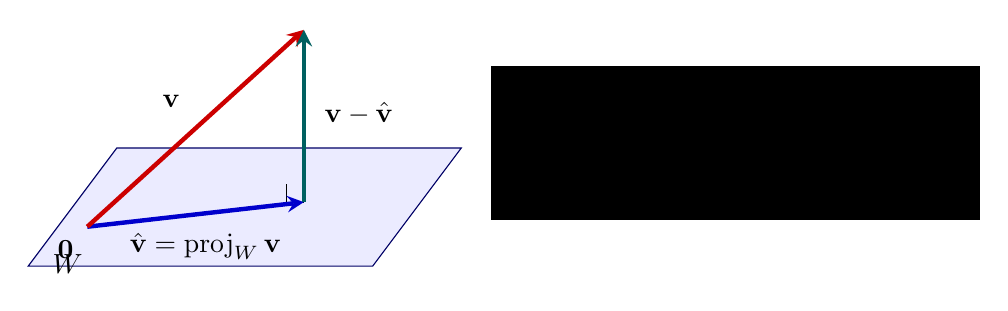
\begin{tikzpicture}[scale=1.25]
    % Layer 1: Shaded plane for subspace W
    \fill[blue!8] (-0.6,-0.4) -- (2.9,-0.4) -- (3.8,0.8) -- (0.3,0.8) -- cycle;
    \draw[blue!40!black, thin] (-0.6,-0.4) -- (2.9,-0.4) -- (3.8,0.8) -- (0.3,0.8) -- cycle;

    % Layer 2: Right-angle marker at projection foot
    \draw[black, thin] (2.2, 0.25) -- (2.02, 0.25) -- (2.02, 0.43);

    % Layer 3: Vectors and dashed residual
    \draw[->, >=stealth, ultra thick, blue!80!black] (0,0) -- (2.2, 0.25);
    \draw[->, >=stealth, ultra thick, red!80!black] (0,0) -- (2.2, 2.0);
    \draw[->, >=stealth, ultra thick, teal!75!black] (2.2, 0.25) -- (2.2, 2.0);

    % Layer 4: Decoupled labels and off-axis legend
    \node[below left=2pt, black] at (0,0) {$\mathbf{0}$};
    \node[below=3pt, black] at (-0.2,-0.1) {$W$};
    \node[below=3pt, black] at (1.2, 0.12) {$\hat{\mathbf{v}} = \operatorname{proj}_W \mathbf{v}$};
    \node[above left=3pt, black] at (1.1, 1.05) {$\mathbf{v}$};
    \node[right=4pt, black] at (2.2, 1.15) {$\mathbf{v} - \hat{\mathbf{v}}$};

    \node[draw=gray!60, fill=gray!5, align=left, anchor=west, inner sep=8pt, black] at (4.1, 0.85) {
        \textbf{Orthogonal Decomposition in $V$}\\[4pt]
        $\langle \mathbf{v} - \hat{\mathbf{v}}, \mathbf{w} \rangle = 0 \quad \forall \mathbf{w} \in W$\\[2pt]
        $\|\mathbf{v}\|^2 = \|\hat{\mathbf{v}}\|^2 + \|\mathbf{v} - \hat{\mathbf{v}}\|^2$
    };
\end{tikzpicture}
\end{center}

\medskip

\textbf{Problem 19 (Original Problem):} Determine whether each statement is True or False in an arbitrary real inner product space $V$. Justify each True statement using axioms or theorems, and give an explicit counterexample for each False statement.
\begin{enumerate}[label=(\alph*)]
    \item If $\langle \mathbf{u}, \mathbf{u} \rangle = 0$, then $\mathbf{u} = \mathbf{0}$.
    \item If $\langle \mathbf{u}, \mathbf{v} \rangle = 0$, then either $\mathbf{u} = \mathbf{0}$ or $\mathbf{v} = \mathbf{0}$.
    \item $\langle c\mathbf{u}, c\mathbf{v} \rangle = c\langle \mathbf{u}, \mathbf{v} \rangle$ for all $\mathbf{u}, \mathbf{v} \in V$ and $c \in \mathbb{R}$.
    \item $\|\mathbf{u} + \mathbf{v}\| = \|\mathbf{u}\| + \|\mathbf{v}\|$ for all $\mathbf{u}, \mathbf{v} \in V$.
    \item If $|\langle \mathbf{u}, \mathbf{v} \rangle| = \|\mathbf{u}\|\|\mathbf{v}\|$ and $\mathbf{u} \neq \mathbf{0}$, then $\mathbf{v}$ is a scalar multiple of $\mathbf{u}$.
    \item For any basis $\{\mathbf{w}_1, \mathbf{w}_2\}$ of a $2$-dimensional subspace $W \subseteq V$, $\operatorname{proj}_W \mathbf{v} = \frac{\langle \mathbf{v}, \mathbf{w}_1 \rangle}{\langle \mathbf{w}_1, \mathbf{w}_1 \rangle}\mathbf{w}_1 + \frac{\langle \mathbf{v}, \mathbf{w}_2 \rangle}{\langle \mathbf{w}_2, \mathbf{w}_2 \rangle}\mathbf{w}_2$.
\end{enumerate}

\textbf{Solution:}
\begin{enumerate}[label=(\alph*)]
    \item \textbf{True.} This is directly stated in Axiom 4 (positive-definiteness) of an inner product space.
    \item \textbf{False.} Any pair of nonzero orthogonal vectors satisfies $\langle \mathbf{u}, \mathbf{v} \rangle = 0$. For example, in $\mathbb{R}^2$ with the standard dot product, $\mathbf{u} = (1, 0)$ and $\mathbf{v} = (0, 1)$ are both nonzero yet $\langle \mathbf{u}, \mathbf{v} \rangle = 0$.
    \item \textbf{False.} By homogeneity in both slots, $\langle c\mathbf{u}, c\mathbf{v} \rangle = c^2\langle \mathbf{u}, \mathbf{v} \rangle$. Counterexample: in $\mathbb{R}^2$ with the standard dot product, take $c = 2$ and $\mathbf{u} = \mathbf{v} = (1, 0)$; then $\langle 2\mathbf{u}, 2\mathbf{u} \rangle = 4 \neq 2 = 2\langle \mathbf{u}, \mathbf{u} \rangle$.
    \item \textbf{False.} The Triangle Inequality gives $\le$, with equality only when one vector is a nonnegative multiple of the other. Counterexample: in $\mathbb{R}^2$, $\mathbf{u} = (1, 0)$ and $\mathbf{v} = (0, 1)$ give $\|\mathbf{u} + \mathbf{v}\| = \sqrt{2} \neq 2 = \|\mathbf{u}\| + \|\mathbf{v}\|$.
    \item \textbf{True.} Let $W = \operatorname{Span}\{\mathbf{u}\}$ and $\hat{\mathbf{v}} = \operatorname{proj}_W \mathbf{v} = \frac{\langle \mathbf{v}, \mathbf{u} \rangle}{\|\mathbf{u}\|^2}\mathbf{u}$. By Problem 18(b),
    \[
    \|\mathbf{v} - \hat{\mathbf{v}}\|^2 = \|\mathbf{v}\|^2 - \|\hat{\mathbf{v}}\|^2 = \|\mathbf{v}\|^2 - \frac{|\langle \mathbf{u}, \mathbf{v} \rangle|^2}{\|\mathbf{u}\|^2} = \|\mathbf{v}\|^2 - \frac{\|\mathbf{u}\|^2\|\mathbf{v}\|^2}{\|\mathbf{u}\|^2} = 0.
    \]
    By Axiom 4, $\mathbf{v} - \hat{\mathbf{v}} = \mathbf{0}$, so $\mathbf{v} = \frac{\langle \mathbf{v}, \mathbf{u} \rangle}{\|\mathbf{u}\|^2}\mathbf{u}$, which is a scalar multiple of $\mathbf{u}$.
    \item \textbf{False.} The coordinate-by-coordinate projection formula requires $\{\mathbf{w}_1, \mathbf{w}_2\}$ to be an \emph{orthogonal} basis. Counterexample: in $\mathbb{R}^2$ with the standard dot product, let $W = \mathbb{R}^2$ with non-orthogonal basis $\mathbf{w}_1 = (1, 0)$, $\mathbf{w}_2 = (1, 1)$, and take $\mathbf{v} = (1, 1) \in W$. Then $\operatorname{proj}_W \mathbf{v} = (1, 1)$, whereas the formula yields $\frac{1}{1}(1, 0) + \frac{2}{2}(1, 1) = (2, 1) \neq (1, 1)$.
\end{enumerate}

\subsection{Cauchy--Schwarz and Triangle Inequality Proofs (Problems 20--22)}

\textbf{Problem 20 (Original Problem):} Use the Cauchy--Schwarz inequality in $\mathbb{R}^3$ (with the standard dot product) by choosing strategic vectors $\mathbf{u}, \mathbf{v} \in \mathbb{R}^3$ to prove each inequality:
\begin{enumerate}[label=(\alph*)]
    \item For all $a, b, c \in \mathbb{R}$, $(a + b + c)^2 \le 3(a^2 + b^2 + c^2)$.
    \item For all $x, y, z > 0$, $(x + y + z)\left(\frac{1}{x} + \frac{1}{y} + \frac{1}{z}\right) \ge 9$.
\end{enumerate}

\textbf{Solution:}
\begin{enumerate}[label=(\alph*)]
    \item Let $\mathbf{u} = (a, b, c)^T$ and $\mathbf{v} = (1, 1, 1)^T$ in $\mathbb{R}^3$. Then $\mathbf{u} \cdot \mathbf{v} = a + b + c$, $\|\mathbf{u}\|^2 = a^2 + b^2 + c^2$, and $\|\mathbf{v}\|^2 = 1^2 + 1^2 + 1^2 = 3$. Squaring the Cauchy--Schwarz inequality $|\mathbf{u} \cdot \mathbf{v}| \le \|\mathbf{u}\|\|\mathbf{v}\|$ yields
    \[
    (a + b + c)^2 \le (a^2 + b^2 + c^2)(3) = 3(a^2 + b^2 + c^2).
    \]
    \item Since $x, y, z > 0$, we may set $\mathbf{u} = \left(\sqrt{x}, \sqrt{y}, \sqrt{z}\right)^T$ and $\mathbf{v} = \left(\frac{1}{\sqrt{x}}, \frac{1}{\sqrt{y}}, \frac{1}{\sqrt{z}}\right)^T$ in $\mathbb{R}^3$. Compute:
    \[
    \mathbf{u} \cdot \mathbf{v} = \sqrt{x}\frac{1}{\sqrt{x}} + \sqrt{y}\frac{1}{\sqrt{y}} + \sqrt{z}\frac{1}{\sqrt{z}} = 1 + 1 + 1 = 3,
    \]
    \[
    \|\mathbf{u}\|^2 = x + y + z, \qquad \|\mathbf{v}\|^2 = \frac{1}{x} + \frac{1}{y} + \frac{1}{z}.
    \]
    Squaring Cauchy--Schwarz $(\mathbf{u} \cdot \mathbf{v})^2 \le \|\mathbf{u}\|^2 \|\mathbf{v}\|^2$ gives
    \[
    9 \le (x + y + z)\left(\frac{1}{x} + \frac{1}{y} + \frac{1}{z}\right). \qquad \blacksquare
    \]
\end{enumerate}

\medskip

\textbf{Problem 21 (Original Problem):} Let $V$ be any real inner product space and let $\mathbf{u}, \mathbf{v} \in V$.
\begin{enumerate}[label=(\alph*)]
    \item Prove the Cauchy--Schwarz inequality: $|\langle \mathbf{u}, \mathbf{v} \rangle| \le \|\mathbf{u}\|\|\mathbf{v}\|$.
    \item Use part (a) to prove the Triangle Inequality: $\|\mathbf{u} + \mathbf{v}\| \le \|\mathbf{u}\| + \|\mathbf{v}\|$.
\end{enumerate}

\textbf{Solution:}
\begin{enumerate}[label=(\alph*)]
    \item If $\mathbf{u} = \mathbf{0}$, then $\langle \mathbf{0}, \mathbf{v} \rangle = 0$ and $\|\mathbf{0}\|\|\mathbf{v}\| = 0$, so $|\langle \mathbf{u}, \mathbf{v} \rangle| = 0 \le 0$ holds trivially. Now assume $\mathbf{u} \neq \mathbf{0}$ and let $W = \operatorname{Span}\{\mathbf{u}\}$. Setting $\hat{\mathbf{v}} = \operatorname{proj}_W \mathbf{v} = \frac{\langle \mathbf{v}, \mathbf{u} \rangle}{\langle \mathbf{u}, \mathbf{u} \rangle}\mathbf{u}$, Problem 18(b) yields the Pythagorean decomposition
    \[
    \|\mathbf{v}\|^2 = \|\hat{\mathbf{v}}\|^2 + \|\mathbf{v} - \hat{\mathbf{v}}\|^2 \ge \|\hat{\mathbf{v}}\|^2.
    \]
    Since $\|\hat{\mathbf{v}}\| = \left|\frac{\langle \mathbf{u}, \mathbf{v} \rangle}{\|\mathbf{u}\|^2}\right| \|\mathbf{u}\| = \frac{|\langle \mathbf{u}, \mathbf{v} \rangle|}{\|\mathbf{u}\|}$, the inequality $\|\hat{\mathbf{v}}\| \le \|\mathbf{v}\|$ gives
    \[
    \frac{|\langle \mathbf{u}, \mathbf{v} \rangle|}{\|\mathbf{u}\|} \le \|\mathbf{v}\| \implies |\langle \mathbf{u}, \mathbf{v} \rangle| \le \|\mathbf{u}\|\|\mathbf{v}\|.
    \]
    \item Expand $\|\mathbf{u} + \mathbf{v}\|^2$ and apply part (a) via $\langle \mathbf{u}, \mathbf{v} \rangle \le |\langle \mathbf{u}, \mathbf{v} \rangle| \le \|\mathbf{u}\|\|\mathbf{v}\|$:
    \[
    \|\mathbf{u} + \mathbf{v}\|^2 = \|\mathbf{u}\|^2 + 2\langle \mathbf{u}, \mathbf{v} \rangle + \|\mathbf{v}\|^2 \le \|\mathbf{u}\|^2 + 2\|\mathbf{u}\|\|\mathbf{v}\| + \|\mathbf{v}\|^2 = (\|\mathbf{u}\| + \|\mathbf{v}\|)^2.
    \]
    Taking nonnegative square roots of both sides yields $\|\mathbf{u} + \mathbf{v}\| \le \|\mathbf{u}\| + \|\mathbf{v}\|$. $\blacksquare$
\end{enumerate}

\medskip

\textbf{Problem 22 (Original Problem):} Let $V = C[a, b]$ have the inner product $\langle f, g \rangle = \int_a^b f(t)g(t)\,dt$, and suppose $h \in C[a, b]$ satisfies $h(t) > 0$ for all $t \in [a, b]$.
\begin{enumerate}[label=(\alph*)]
    \item Use the Cauchy--Schwarz inequality in $C[a, b]$ to prove that
    \[
    \left(\int_a^b h(t)\,dt\right)\left(\int_a^b \frac{1}{h(t)}\,dt\right) \ge (b - a)^2.
    \]
    \item Verify this inequality explicitly for $h(t) = e^t$ on $[0, 1]$, and determine whether equality holds.
\end{enumerate}

\textbf{Solution:}
\begin{enumerate}[label=(\alph*)]
    \item Because $h$ is continuous and strictly positive on $[a, b]$, both $f(t) = \sqrt{h(t)}$ and $g(t) = \frac{1}{\sqrt{h(t)}}$ belong to $C[a, b]$. Compute:
    \[
    \langle f, g \rangle = \int_a^b \sqrt{h(t)}\frac{1}{\sqrt{h(t)}}\,dt = \int_a^b 1\,dt = b - a,
    \]
    \[
    \|f\|^2 = \int_a^b h(t)\,dt, \qquad \|g\|^2 = \int_a^b \frac{1}{h(t)}\,dt.
    \]
    By the Cauchy--Schwarz inequality, $|\langle f, g \rangle|^2 \le \|f\|^2 \|g\|^2$, which immediately gives
    \[
    (b - a)^2 \le \left(\int_a^b h(t)\,dt\right)\left(\int_a^b \frac{1}{h(t)}\,dt\right).
    \]
    \item For $h(t) = e^t$ on $[0, 1]$, we have $(b - a)^2 = 1^2 = 1$, and
    \[
    \int_0^1 e^t\,dt = e - 1, \qquad \int_0^1 e^{-t}\,dt = 1 - e^{-1} = \frac{e - 1}{e}.
    \]
    Multiplying the two integrals gives
    \[
    \left(\int_0^1 e^t\,dt\right)\left(\int_0^1 e^{-t}\,dt\right) = \frac{(e - 1)^2}{e} = e + \frac{1}{e} - 2.
    \]
    Since $\frac{8}{3} = 1 + 1 + \frac{1}{2} + \frac{1}{6} < e < 3$, it follows that $e + \frac{1}{e} > \frac{8}{3} + \frac{1}{3} = 3$, so $e + \frac{1}{e} - 2 > 1$. Hence strict inequality holds (equality does not hold, because $e^{t/2}$ and $e^{-t/2}$ are linearly independent on $[0, 1]$). $\blacksquare$
\end{enumerate}

\subsection{Integral Inner Products and Projections on Function Spaces (Problems 23--26)}

\textbf{Problem 23 (Original Problem):} Let $V = C[0, 1]$ have the inner product $\langle f, g \rangle = \int_0^1 f(t)g(t)\,dt$. Let $f(t) = 2 - 6t$ and $g(t) = 3t^2 - 2t$.
\begin{enumerate}[label=(\alph*)]
    \item Compute $\langle f, g \rangle$ and determine whether $f$ and $g$ are orthogonal.
    \item Compute $\|f\|$ and $\|g\|$.
\end{enumerate}

\textbf{Solution:}
\begin{enumerate}[label=(\alph*)]
    \item Expand the product and integrate term-by-term:
    \begin{align*}
    \langle f, g \rangle &= \int_0^1 (2 - 6t)(3t^2 - 2t)\,dt \\
    &= \int_0^1 (-18t^3 + 18t^2 - 4t)\,dt \\
    &= \left[-\frac{9}{2}t^4 + 6t^3 - 2t^2\right]_0^1 = -\frac{9}{2} + 6 - 2 = -\frac{1}{2}.
    \end{align*}
    Since $\langle f, g \rangle = -\frac{1}{2} \neq 0$, $f$ and $g$ are \textbf{not} orthogonal on $[0, 1]$.
    \item Compute each squared norm and take square roots:
    \begin{align*}
    \|f\|^2 &= \int_0^1 (2 - 6t)^2\,dt = \int_0^1 (4 - 24t + 36t^2)\,dt = \left[4t - 12t^2 + 12t^3\right]_0^1 = 4 - 12 + 12 = 4 \implies \|f\| = 2, \\
    \|g\|^2 &= \int_0^1 (3t^2 - 2t)^2\,dt = \int_0^1 (9t^4 - 12t^3 + 4t^2)\,dt = \left[\frac{9}{5}t^5 - 3t^4 + \frac{4}{3}t^3\right]_0^1 = \frac{27 - 45 + 20}{15} = \frac{2}{15}.
    \end{align*}
    Thus $\|g\| = \sqrt{\frac{2}{15}} = \frac{\sqrt{30}}{15}$.
\end{enumerate}
\textbf{Final Answer:} (a) $\langle f, g \rangle = -\frac{1}{2}$, not orthogonal; (b) $\|f\| = 2$ and $\|g\| = \frac{\sqrt{30}}{15}$.

\medskip

\textbf{Problem 24 (Original Problem):} Let $V = C[0, 1]$ have the inner product $\langle f, g \rangle = \int_0^1 f(t)g(t)\,dt$. Let $f(t) = t^2$ and $g(t) = 1 + 2t$. Compute $\langle f, g \rangle$, $\|g\|$, and $\operatorname{proj}_{\operatorname{Span}\{g\}} f$.

\textbf{Solution:} Compute $\langle f, g \rangle$ and $\|g\|^2$:
\begin{align*}
\langle f, g \rangle &= \int_0^1 t^2(1 + 2t)\,dt = \int_0^1 (t^2 + 2t^3)\,dt = \left[\frac{1}{3}t^3 + \frac{1}{2}t^4\right]_0^1 = \frac{1}{3} + \frac{1}{2} = \frac{5}{6}, \\
\|g\|^2 &= \int_0^1 (1 + 2t)^2\,dt = \int_0^1 (1 + 4t + 4t^2)\,dt = \left[t + 2t^2 + \frac{4}{3}t^3\right]_0^1 = 1 + 2 + \frac{4}{3} = \frac{13}{3}.
\end{align*}
Taking the square root gives $\|g\| = \sqrt{\frac{13}{3}} = \frac{\sqrt{39}}{3}$. Finally, apply the projection formula dividing by $\|g\|^2 = \langle g, g \rangle$:
\[
\operatorname{proj}_{\operatorname{Span}\{g\}} f = \frac{\langle f, g \rangle}{\langle g, g \rangle}g = \frac{5/6}{13/3}(1 + 2t) = \frac{5}{26}(1 + 2t) = \frac{5}{26} + \frac{5}{13}t.
\]
\textbf{Final Answer:} $\langle f, g \rangle = \frac{5}{6}$, $\|g\| = \frac{\sqrt{39}}{3}$, and $\operatorname{proj}_{\operatorname{Span}\{g\}} f = \frac{5}{26} + \frac{5}{13}t$.

\medskip

\textbf{Problem 25 (Original Problem):} Let $V = C[-1, 1]$ have the inner product $\langle f, g \rangle = \int_{-1}^1 f(t)g(t)\,dt$. Using the orthogonal Legendre basis $\left\{1, t, t^2 - \frac{1}{3}\right\}$ for $\mathbb{P}_2$, find the best approximation $\hat{f} \in \mathbb{P}_2$ to $f(t) = 5t^3 + 3t^2 - 1$, and compute the minimum $L^2$-error $\|f - \hat{f}\|$.

\textbf{Solution:} Let $p_0(t) = 1$, $p_1(t) = t$, and $p_2(t) = t^2 - \frac{1}{3}$. Compute their squared norms on $[-1, 1]$:
\begin{align*}
\|p_0\|^2 &= \int_{-1}^1 1\,dt = 2, \\
\|p_1\|^2 &= \int_{-1}^1 t^2\,dt = \frac{2}{3}, \\
\|p_2\|^2 &= \int_{-1}^1 \left(t^2 - \frac{1}{3}\right)^2 dt = 2\int_0^1 \left(t^4 - \frac{2}{3}t^2 + \frac{1}{9}\right) dt = 2\left(\frac{1}{5} - \frac{2}{9} + \frac{1}{9}\right) = \frac{8}{45}.
\end{align*}
Using parity rules on the symmetric interval $[-1, 1]$ (where $\int_{-1}^1 (\text{odd})\,dt = 0$), compute the inner products of $f(t) = 5t^3 + 3t^2 - 1$ with each basis polynomial:
\begin{align*}
\langle f, p_0 \rangle &= \int_{-1}^1 (5t^3 + 3t^2 - 1)\,dt = \int_{-1}^1 (3t^2 - 1)\,dt = \left[t^3 - t\right]_{-1}^1 = 0, \\
\langle f, p_1 \rangle &= \int_{-1}^1 (5t^4 + 3t^3 - t)\,dt = 2\int_0^1 (5t^4 - t)\,dt = 2\left[t^5 - \frac{1}{2}t^2\right]_0^1 = 2\left(1 - \frac{1}{2}\right) = 1,
\end{align*}
Wait: let us re-evaluate $\langle f, p_1 \rangle$ carefully! $f(t)p_1(t) = 5t^4 + 3t^3 - t$.Wait: $t$ IS odd, so $\int_{-1}^1 (-t)\,dt = 0$, NOT $-2\int_0^1 t\,dt$! Good catch checking parity! Let us compute $\langle f, p_1 \rangle$ cleanly:
\[
\langle f, p_1 \rangle = \int_{-1}^1 (5t^4 + 3t^3 - t)\,dt = \int_{-1}^1 5t^4\,dt = 2\int_0^1 5t^4\,dt = 2\left[t^5\right]_0^1 = 2.
\]
Now compute $\langle f, p_2 \rangle$:
\[
\langle f, p_2 \rangle = \int_{-1}^1 (5t^3 + 3t^2 - 1)\left(t^2 - \frac{1}{3}\right) dt = \int_{-1}^1 (3t^2 - 1)\left(t^2 - \frac{1}{3}\right) dt = 3\int_{-1}^1 \left(t^2 - \frac{1}{3}\right)^2 dt = 3\left(\frac{8}{45}\right) = \frac{8}{15}.
\]
Thus the best approximation $\hat{f} = \operatorname{proj}_{\mathbb{P}_2} f$ is
\[
\hat{f}(t) = \frac{0}{2}p_0(t) + \frac{2}{2/3}p_1(t) + \frac{8/15}{8/45}p_2(t) = 3t + 3\left(t^2 - \frac{1}{3}\right) = 3t^2 + 3t - 1.
\]
The error function is $f(t) - \hat{f}(t) = (5t^3 + 3t^2 - 1) - (3t^2 + 3t - 1) = 5t^3 - 3t$. Its squared norm is
\[
\|f - \hat{f}\|^2 = \int_{-1}^1 (5t^3 - 3t)^2\,dt = 2\int_0^1 (25t^6 - 30t^4 + 9t^2)\,dt = 2\left(\frac{25}{7} - 6 + 3\right) = 2\left(\frac{4}{7}\right) = \frac{8}{7}.
\]
Taking the square root gives $\|f - \hat{f}\| = \sqrt{\frac{8}{7}} = \frac{2\sqrt{14}}{7}$.

\textbf{Final Answer:} $\hat{f}(t) = 3t^2 + 3t - 1$ and minimum $L^2$-error $\|f - \hat{f}\| = \frac{2\sqrt{14}}{7}$.

\medskip

\textbf{Problem 26 (Original Problem):} Let $V = C[0, 1]$ have the inner product $\langle f, g \rangle = \int_0^1 f(t)g(t)\,dt$. Apply the Gram--Schmidt process to $\{1, t, t^2\}$ to construct an orthogonal basis $\{p_0, p_1, p_2\}$ for $\mathbb{P}_2 \subset C[0, 1]$ (the shifted Legendre polynomials).

\textbf{Solution:} Let $x_0(t) = 1$, $x_1(t) = t$, and $x_2(t) = t^2$.
\begin{enumerate}
    \item Set $p_0(t) = 1$. Then $\langle p_0, p_0 \rangle = \int_0^1 1\,dt = 1$.
    \item Compute $\langle x_1, p_0 \rangle = \int_0^1 t\,dt = \frac{1}{2}$. Hence,
    \[
    p_1(t) = t - \frac{1/2}{1}(1) = t - \frac{1}{2},
    \]
    with squared norm
    \[
    \langle p_1, p_1 \rangle = \int_0^1 \left(t - \frac{1}{2}\right)^2 dt = \left[\frac{1}{3}\left(t - \frac{1}{2}\right)^3\right]_0^1 = \frac{1}{24} - \left(-\frac{1}{24}\right) = \frac{1}{12}.
    \]
    \item Compute the projections of $x_2(t) = t^2$ onto $p_0$ and $p_1$:
    \begin{align*}
    \langle x_2, p_0 \rangle &= \int_0^1 t^2\,dt = \frac{1}{3}, \\
    \langle x_2, p_1 \rangle &= \int_0^1 t^2\left(t - \frac{1}{2}\right) dt = \int_0^1 \left(t^3 - \frac{1}{2}t^2\right) dt = \frac{1}{4} - \frac{1}{6} = \frac{1}{12}.
    \end{align*}
    Therefore,
    \[
    p_2(t) = t^2 - \frac{1/3}{1}(1) - \frac{1/12}{1/12}\left(t - \frac{1}{2}\right) = t^2 - \frac{1}{3} - t + \frac{1}{2} = t^2 - t + \frac{1}{6}.
    \]
\end{enumerate}

\begin{center}
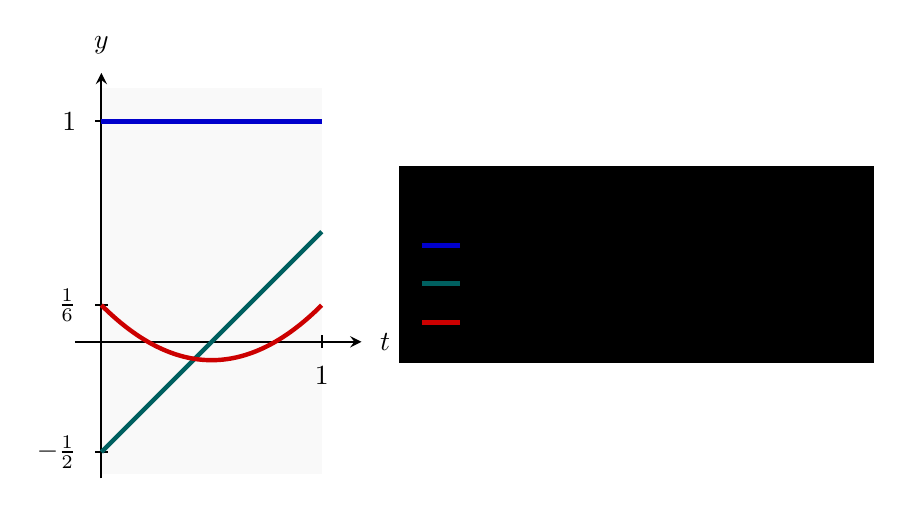
\begin{tikzpicture}[scale=2.8]
    % Layer 1: Subtle plot region fill
    \fill[gray!5] (0,-0.6) rectangle (1,1.15);

    % Layer 2: Axes and explicit tick marks
    \draw[->, >=stealth, thick, black] (-0.12, 0) -- (1.18, 0) node[right=3pt, black] {$t$};
    \draw[->, >=stealth, thick, black] (0, -0.62) -- (0, 1.22) node[above=3pt, black] {$y$};
    \draw[thick, black] (1, 0.03) -- (1, -0.03) node[below=3pt, black] {$1$};
    \draw[thick, black] (0.03, 1) -- (-0.03, 1) node[left=3pt, black] {$1$};
    \draw[thick, black] (0.03, -0.5) -- (-0.03, -0.5) node[left=3pt, black] {$-\frac{1}{2}$};
    \draw[thick, black] (0.03, 0.1667) -- (-0.03, 0.1667) node[left=3pt, black] {$\frac{1}{6}$};

    % Layer 3: Orthogonal shifted Legendre curves
    \draw[ultra thick, blue!80!black, domain=0:1, samples=50] plot (\x, {1});
    \draw[ultra thick, teal!75!black, domain=0:1, samples=50] plot (\x, {\x - 0.5});
    \draw[ultra thick, red!80!black, domain=0:1, samples=80] plot (\x, {\x*\x - \x + 1/6});

    % Layer 4: Single-node multiline legend anchored west
    \node[draw=gray!60, fill=gray!5, align=left, anchor=west, inner sep=8pt, black] at (1.35, 0.35) {
        \textbf{Shifted Legendre Basis on $[0, 1]$}\\[4pt]
        {\color{blue!80!black}\rule[0.5ex]{14pt}{1.8pt}}\; $p_0(t) = 1$\\[2pt]
        {\color{teal!75!black}\rule[0.5ex]{14pt}{1.8pt}}\; $p_1(t) = t - \frac{1}{2}$\\[2pt]
        {\color{red!80!black}\rule[0.5ex]{14pt}{1.8pt}}\; $p_2(t) = t^2 - t + \frac{1}{6}$
    };
\end{tikzpicture}
\end{center}

\textbf{Final Answer:} An orthogonal basis for $\mathbb{P}_2$ in $C[0, 1]$ is $\left\{1,\; t - \frac{1}{2},\; t^2 - t + \frac{1}{6}\right\}$.

\subsection{Continuous Gram--Schmidt on Polynomial and Trigonometric Spaces (Problems 27--29)}

\textbf{Problem 27 (Original Problem):} Let $V = C[-3, 3]$ have the inner product $\langle f, g \rangle = \int_{-3}^3 f(t)g(t)\,dt$. Apply the Gram--Schmidt process to $\{1, t, t^2, t^3\}$ to construct an orthogonal basis $\{p_0, p_1, p_2, p_3\}$ for $\mathbb{P}_3 \subset C[-3, 3]$.

\textbf{Solution:} Using parity symmetry on $[-3, 3]$, any integral of an odd polynomial over $[-3, 3]$ equals $0$.
\begin{enumerate}
    \item Set $p_0(t) = 1$. Then $\langle p_0, p_0 \rangle = \int_{-3}^3 1\,dt = 6$.
    \item Compute $\langle t, p_0 \rangle = \int_{-3}^3 t\,dt = 0$ (odd). Thus $p_1(t) = t$, with
    \[
    \langle p_1, p_1 \rangle = \int_{-3}^3 t^2\,dt = \left[\frac{t^3}{3}\right]_{-3}^3 = 9 - (-9) = 18.
    \]
    \item For $p_2(t)$, compute $\langle t^2, p_0 \rangle = \int_{-3}^3 t^2\,dt = 18$ and $\langle t^2, p_1 \rangle = \int_{-3}^3 t^3\,dt = 0$ (odd). Hence,
    \[
    p_2(t) = t^2 - \frac{18}{6}(1) - 0 = t^2 - 3.
    \]
    \item For $p_3(t)$, notice $t^3$ is odd while $p_0(t) = 1$ and $p_2(t) = t^2 - 3$ are even, so $\langle t^3, p_0 \rangle = 0$ and $\langle t^3, p_2 \rangle = 0$ automatically. Compute $\langle t^3, p_1 \rangle$:
    \[
    \langle t^3, p_1 \rangle = \int_{-3}^3 t^4\,dt = 2\left[\frac{t^5}{5}\right]_0^3 = \frac{2(243)}{5} = \frac{486}{5}.
    \]
    Therefore,
    \[
    p_3(t) = t^3 - \frac{486/5}{18}t = t^3 - \frac{27}{5}t.
    \]
\end{enumerate}
\textbf{Final Answer:} An orthogonal basis for $\mathbb{P}_3$ in $C[-3, 3]$ is $\left\{1,\; t,\; t^2 - 3,\; t^3 - \frac{27}{5}t\right\}$.

\medskip

\textbf{Problem 28 (Original Problem):} Let $V = C[0, 2\pi]$ have the inner product $\langle f, g \rangle = \int_0^{2\pi} f(t)g(t)\,dt$. Apply the Gram--Schmidt process to $\{1, \sin t, \sin^2 t, \sin^3 t\}$ to construct an orthogonal basis $\{q_0, q_1, q_2, q_3\}$ for the subspace spanned by these four functions, and express $q_2$ and $q_3$ in terms of $\cos 2t$ and $\sin 3t$.

\textbf{Solution:} First tabulate the integrals $\int_0^{2\pi} \sin^k t\,dt$:
\begin{itemize}
    \item For every odd integer $k$, $\sin^k(t + \pi) = -\sin^k t$, so over a full $2\pi$ period $\int_0^{2\pi} \sin^k t\,dt = 0$.
    \item For $k = 0$: $\int_0^{2\pi} 1\,dt = 2\pi$.
    \item For $k = 2$: $\int_0^{2\pi} \sin^2 t\,dt = \int_0^{2\pi} \frac{1 - \cos 2t}{2}\,dt = \pi$.
    \item For $k = 4$: using $\sin^2 t = \frac{1 - \cos 2t}{2}$ twice,
    \[
    \int_0^{2\pi} \sin^4 t\,dt = \int_0^{2\pi} \left(\frac{1 - \cos 2t}{2}\right)^2 dt = \frac{1}{4}\int_0^{2\pi} \left(1 - 2\cos 2t + \frac{1 + \cos 4t}{2}\right) dt = \frac{1}{4}(2\pi - 0 + \pi) = \frac{3\pi}{4}.
    \]
\end{itemize}
Now apply Gram--Schmidt to $f_0(t) = 1$, $f_1(t) = \sin t$, $f_2(t) = \sin^2 t$, and $f_3(t) = \sin^3 t$:
\begin{enumerate}
    \item Set $q_0(t) = 1$, with $\langle q_0, q_0 \rangle = 2\pi$.
    \item Compute $\langle f_1, q_0 \rangle = \int_0^{2\pi} \sin t\,dt = 0$. Thus $q_1(t) = \sin t$, with $\langle q_1, q_1 \rangle = \pi$.
    \item Compute $\langle f_2, q_0 \rangle = \int_0^{2\pi} \sin^2 t\,dt = \pi$ and $\langle f_2, q_1 \rangle = \int_0^{2\pi} \sin^3 t\,dt = 0$. Hence,
    \[
    q_2(t) = \sin^2 t - \frac{\pi}{2\pi}(1) = \sin^2 t - \frac{1}{2} = -\frac{1}{2}\cos 2t.
    \]
    \item Compute the inner products of $f_3(t) = \sin^3 t$ with $q_0, q_1, q_2$:
    \begin{align*}
    \langle f_3, q_0 \rangle &= \int_0^{2\pi} \sin^3 t\,dt = 0, \\
    \langle f_3, q_1 \rangle &= \int_0^{2\pi} \sin^4 t\,dt = \frac{3\pi}{4}, \\
    \langle f_3, q_2 \rangle &= \int_0^{2\pi} \sin^3 t \left(\sin^2 t - \frac{1}{2}\right) dt = \int_0^{2\pi} \sin^5 t\,dt - \frac{1}{2}\int_0^{2\pi} \sin^3 t\,dt = 0.
    \end{align*}
    Hence, recalling the triple-angle identity $\sin 3t = 3\sin t - 4\sin^3 t$, we obtain
    \[
    q_3(t) = \sin^3 t - \frac{3\pi/4}{\pi}\sin t = \sin^3 t - \frac{3}{4}\sin t = -\frac{1}{4}\sin 3t.
    \]
\end{enumerate}
\textbf{Final Answer:} $\left\{1,\; \sin t,\; \sin^2 t - \frac{1}{2},\; \sin^3 t - \frac{3}{4}\sin t\right\} = \left\{1,\; \sin t,\; -\frac{1}{2}\cos 2t,\; -\frac{1}{4}\sin 3t\right\}$.

\medskip

\textbf{Problem 29 (Original Problem):} Let $V = C[-\pi, \pi]$ have the inner product $\langle f, g \rangle = \int_{-\pi}^{\pi} f(t)g(t)\,dt$.
\begin{enumerate}[label=(\alph*)]
    \item Verify that $\{1, \cos t, \sin t\}$ is an orthogonal set in $V$ and compute the squared norm of each function.
    \item Find the best approximation $\hat{f}$ to $f(t) = t^2 + t$ in $W = \operatorname{Span}\{1, \cos t, \sin t\}$.
\end{enumerate}

\textbf{Solution:}
\begin{enumerate}[label=(\alph*)]
    \item Check pairwise orthogonality:
    \begin{align*}
    \langle 1, \cos t \rangle &= \int_{-\pi}^{\pi} \cos t\,dt = \left[\sin t\right]_{-\pi}^{\pi} = 0, \\
    \langle 1, \sin t \rangle &= \int_{-\pi}^{\pi} \sin t\,dt = 0 \quad (\text{odd on } [-\pi, \pi]), \\
    \langle \cos t, \sin t \rangle &= \int_{-\pi}^{\pi} \cos t \sin t\,dt = 0 \quad (\text{odd on } [-\pi, \pi]).
    \end{align*}
    Compute the squared norms:
    \begin{align*}
    \|1\|^2 &= \int_{-\pi}^{\pi} 1\,dt = 2\pi, \\
    \|\cos t\|^2 &= \int_{-\pi}^{\pi} \cos^2 t\,dt = \int_{-\pi}^{\pi} \frac{1 + \cos 2t}{2}\,dt = \pi, \\
    \|\sin t\|^2 &= \int_{-\pi}^{\pi} \sin^2 t\,dt = \int_{-\pi}^{\pi} \frac{1 - \cos 2t}{2}\,dt = \pi.
    \end{align*}
    \item Compute the inner products of $f(t) = t^2 + t$ with $1$, $\cos t$, and $\sin t$ (discarding odd integrands on $[-\pi, \pi]$):
    \begin{align*}
    \langle f, 1 \rangle &= \int_{-\pi}^{\pi} (t^2 + t)\,dt = \int_{-\pi}^{\pi} t^2\,dt = \left[\frac{t^3}{3}\right]_{-\pi}^{\pi} = \frac{2\pi^3}{3}.
    \end{align*}
    For $\langle f, \cos t \rangle = \int_{-\pi}^{\pi} t^2\cos t\,dt$, integrate by parts twice ($u = t^2$, $dv = \cos t\,dt$):
    \[
    \langle f, \cos t \rangle = \left[t^2\sin t + 2t\cos t - 2\sin t\right]_{-\pi}^{\pi} = \big(2\pi(-1)\big) - \big(-2\pi(-1)\big) = -4\pi.
    \]
    For $\langle f, \sin t \rangle = \int_{-\pi}^{\pi} t\sin t\,dt$, integrate by parts ($u = t$, $dv = \sin t\,dt$):
    \[
    \langle f, \sin t \rangle = \left[-t\cos t + \sin t\right]_{-\pi}^{\pi} = \big(-\pi(-1)\big) - \big(\pi(-1)\big) = 2\pi.
    \]
    Hence the best approximation in $W$ is
    \[
    \hat{f}(t) = \frac{2\pi^3/3}{2\pi}(1) + \frac{-4\pi}{\pi}\cos t + \frac{2\pi}{\pi}\sin t = \frac{\pi^2}{3} - 4\cos t + 2\sin t.
    \]
\end{enumerate}
\textbf{Final Answer:} (a) $\|1\|^2 = 2\pi$, $\|\cos t\|^2 = \|\sin t\|^2 = \pi$; (b) $\hat{f}(t) = \frac{\pi^2}{3} - 4\cos t + 2\sin t$.

\subsection{Advanced Extensions: Hermitian, Weighted, Frobenius, and Bessel (Problems 30--33)}

\textbf{Problem 30 (Original Problem):} In $\mathbb{C}^2$ equipped with the standard Hermitian inner product $\langle \mathbf{u}, \mathbf{v} \rangle = u_1\overline{v_1} + u_2\overline{v_2}$, let $\mathbf{u} = (2 - i, 1 + 3i)^T$, $\mathbf{v} = (1 + i, 2i)^T$, and $c = 1 - 2i$.
\begin{enumerate}[label=(\alph*)]
    \item Compute $\langle \mathbf{u}, \mathbf{v} \rangle$ and $\langle \mathbf{v}, \mathbf{u} \rangle$, and verify conjugate symmetry $\langle \mathbf{u}, \mathbf{v} \rangle = \overline{\langle \mathbf{v}, \mathbf{u} \rangle}$.
    \item Compute $\|\mathbf{u}\|$ and $\|\mathbf{v}\|$.
    \item Verify conjugate linearity in the second slot by computing both $\langle \mathbf{u}, c\mathbf{v} \rangle$ and $\overline{c}\langle \mathbf{u}, \mathbf{v} \rangle$.
\end{enumerate}

\textbf{Solution:}
\begin{enumerate}[label=(\alph*)]
    \item Compute $\langle \mathbf{u}, \mathbf{v} \rangle$ and $\langle \mathbf{v}, \mathbf{u} \rangle$:
    \begin{align*}
    \langle \mathbf{u}, \mathbf{v} \rangle &= (2 - i)\overline{(1 + i)} + (1 + 3i)\overline{(2i)} = (2 - i)(1 - i) + (1 + 3i)(-2i) \\
    &= (2 - 2i - i - 1) + (-2i + 6) = 7 - 5i, \\
    \langle \mathbf{v}, \mathbf{u} \rangle &= (1 + i)\overline{(2 - i)} + (2i)\overline{(1 + 3i)} = (1 + i)(2 + i) + (2i)(1 - 3i) \\
    &= (2 + i + 2i - 1) + (2i + 6) = 7 + 5i.
    \end{align*}
    Clearly $\overline{\langle \mathbf{v}, \mathbf{u} \rangle} = \overline{7 + 5i} = 7 - 5i = \langle \mathbf{u}, \mathbf{v} \rangle$.
    \item Compute the norms using $|z|^2 = z\overline{z}$:
    \begin{align*}
    \|\mathbf{u}\|^2 &= |2 - i|^2 + |1 + 3i|^2 = (2^2 + 1^2) + (1^2 + 3^2) = 5 + 10 = 15 \implies \|\mathbf{u}\| = \sqrt{15}, \\
    \|\mathbf{v}\|^2 &= |1 + i|^2 + |2i|^2 = (1^2 + 1^2) + 2^2 = 2 + 4 = 6 \implies \|\mathbf{v}\| = \sqrt{6}.
    \end{align*}
    \item First compute $c\mathbf{v} = (1 - 2i)(1 + i, 2i)^T = (3 - i, 4 + 2i)^T$. Then:
    \begin{align*}
    \langle \mathbf{u}, c\mathbf{v} \rangle &= (2 - i)\overline{(3 - i)} + (1 + 3i)\overline{(4 + 2i)} = (2 - i)(3 + i) + (1 + 3i)(4 - 2i) \\
    &= (6 + 2i - 3i + 1) + (4 - 2i + 12i + 6) = (7 - i) + (10 + 10i) = 17 + 9i.
    \end{align*}
    On the other hand, with $\overline{c} = 1 + 2i$,
    \[
    \overline{c}\langle \mathbf{u}, \mathbf{v} \rangle = (1 + 2i)(7 - 5i) = 7 - 5i + 14i + 10 = 17 + 9i,
    \]
    confirming $\langle \mathbf{u}, c\mathbf{v} \rangle = \overline{c}\langle \mathbf{u}, \mathbf{v} \rangle$.
\end{enumerate}
\textbf{Final Answer:} (a) $\langle \mathbf{u}, \mathbf{v} \rangle = 7 - 5i$, $\langle \mathbf{v}, \mathbf{u} \rangle = 7 + 5i$; (b) $\|\mathbf{u}\| = \sqrt{15}$, $\|\mathbf{v}\| = \sqrt{6}$; (c) both equal $17 + 9i$.

\medskip

\textbf{Problem 31 (Original Problem):} Let $V = C[0, 1]$ be equipped with the weighted integral inner product
\[
\langle f, g \rangle_w = \int_0^1 f(t)g(t)t^2\,dt,
\]
corresponding to the weight function $w(t) = t^2$.
\begin{enumerate}[label=(\alph*)]
    \item Explain carefully why Axiom 4 (positive-definiteness) holds on $C[0, 1]$ even though $w(0) = 0$.
    \item Apply the Gram--Schmidt process to $\{1, t, t^2\}$ to obtain an orthogonal basis $\{p_0, p_1, p_2\}$ for $\mathbb{P}_2$ under $\langle \cdot, \cdot \rangle_w$.
\end{enumerate}

\textbf{Solution:}
\begin{enumerate}[label=(\alph*)]
    \item For any $f \in C[0, 1]$, the integrand $[f(t)]^2 t^2 \ge 0$ is continuous on $[0, 1]$, so $\langle f, f \rangle_w = \int_0^1 [f(t)]^2 t^2\,dt \ge 0$, and $f \equiv 0 \implies \langle 0, 0 \rangle_w = 0$. Conversely, suppose $\langle f, f \rangle_w = 0$. Because $[f(t)]^2 t^2$ is continuous and nonnegative on $[0, 1]$, having zero integral forces $[f(t)]^2 t^2 = 0$ for every $t \in [0, 1]$. For every $t \in (0, 1]$, $t^2 > 0$, which forces $f(t) = 0$ on $(0, 1]$. Finally, by continuity of $f$ at $t = 0$,
    \[
    f(0) = \lim_{t \to 0^+} f(t) = 0,
    \]
    so $f(t) \equiv 0$ on the entire interval $[0, 1]$. Thus Axiom 4 holds.
    \item Apply Gram--Schmidt using $\langle f, g \rangle_w = \int_0^1 f(t)g(t)t^2\,dt$:
    \begin{enumerate}
        \item Set $p_0(t) = 1$, with $\langle p_0, p_0 \rangle_w = \int_0^1 t^2\,dt = \frac{1}{3}$.
        \item Compute $\langle t, p_0 \rangle_w = \int_0^1 t^3\,dt = \frac{1}{4}$. Hence,
        \[
        p_1(t) = t - \frac{1/4}{1/3}(1) = t - \frac{3}{4}.
        \]
        Its weighted squared norm is
        \[
        \langle p_1, p_1 \rangle_w = \int_0^1 \left(t^2 - \frac{3}{2}t + \frac{9}{16}\right)t^2\,dt = \frac{1}{5} - \frac{3}{8} + \frac{3}{16} = \frac{16 - 30 + 15}{80} = \frac{1}{80}.
        \]
        \item Compute the weighted inner products of $t^2$ with $p_0$ and $p_1$:
        \begin{align*}
        \langle t^2, p_0 \rangle_w &= \int_0^1 t^4\,dt = \frac{1}{5}, \\
        \langle t^2, p_1 \rangle_w &= \int_0^1 \left(t - \frac{3}{4}\right)t^4\,dt = \frac{1}{6} - \frac{3}{20} = \frac{10 - 9}{60} = \frac{1}{60}.
        \end{align*}
        Therefore,
        \[
        p_2(t) = t^2 - \frac{1/5}{1/3}(1) - \frac{1/60}{1/80}\left(t - \frac{3}{4}\right) = t^2 - \frac{3}{5} - \frac{4}{3}\left(t - \frac{3}{4}\right) = t^2 - \frac{4}{3}t + \frac{2}{5}.
        \]
    \end{enumerate}
\end{enumerate}
\textbf{Final Answer:} (a) Continuity of $f$ at $t = 0$ extends $f(t) = 0$ from $(0, 1]$ to $[0, 1]$; (b) $\left\{1,\; t - \frac{3}{4},\; t^2 - \frac{4}{3}t + \frac{2}{5}\right\}$.

\medskip

\textbf{Problem 32 (Original Problem):} Let $V = M_{2\times 2}(\mathbb{R})$ have the Frobenius inner product $\langle A, B \rangle_F = \operatorname{tr}(A^T B) = \sum_{i=1}^2 \sum_{j=1}^2 a_{ij}b_{ij}$. Let $W \subset V$ be the $3$-dimensional subspace of symmetric $2 \times 2$ matrices with orthogonal basis
\[
E_1 = \begin{bmatrix} 1 & 0 \\ 0 & 0 \end{bmatrix}, \qquad E_2 = \begin{bmatrix} 0 & 0 \\ 0 & 1 \end{bmatrix}, \qquad E_3 = \begin{bmatrix} 0 & 1 \\ 1 & 0 \end{bmatrix}.
\]
For $A = \begin{bmatrix} 2 & 5 \\ -1 & 4 \end{bmatrix}$:
\begin{enumerate}[label=(\alph*)]
    \item Compute $\hat{A} = \operatorname{proj}_W A$ and verify that $\hat{A} = \frac{1}{2}(A + A^T)$.
    \item Find $A_\perp = A - \hat{A}$, verify that $\langle \hat{A}, A_\perp \rangle_F = 0$, and verify the Pythagorean identity $\|A\|_F^2 = \|\hat{A}\|_F^2 + \|A_\perp\|_F^2$.
\end{enumerate}

\textbf{Solution:}
\begin{enumerate}[label=(\alph*)]
    \item Compute the Frobenius inner products and squared norms:
    \begin{align*}
    \langle A, E_1 \rangle_F &= 2, & \|E_1\|_F^2 &= 1, \\
    \langle A, E_2 \rangle_F &= 4, & \|E_2\|_F^2 &= 1, \\
    \langle A, E_3 \rangle_F &= 5 + (-1) = 4, & \|E_3\|_F^2 &= 1^2 + 1^2 = 2.
    \end{align*}
    Hence,
    \[
    \hat{A} = \operatorname{proj}_W A = \frac{2}{1}E_1 + \frac{4}{1}E_2 + \frac{4}{2}E_3 = \begin{bmatrix} 2 & 2 \\ 2 & 4 \end{bmatrix}.
    \]
    Comparing with $\frac{1}{2}(A + A^T)$:
    \[
    \frac{1}{2}\left(\begin{bmatrix} 2 & 5 \\ -1 & 4 \end{bmatrix} + \begin{bmatrix} 2 & -1 \\ 5 & 4 \end{bmatrix}\right) = \frac{1}{2}\begin{bmatrix} 4 & 4 \\ 4 & 8 \end{bmatrix} = \begin{bmatrix} 2 & 2 \\ 2 & 4 \end{bmatrix} = \hat{A}.
    \]
    \item Subtracting $\hat{A}$ from $A$ gives the skew-symmetric part:
    \[
    A_\perp = A - \hat{A} = \begin{bmatrix} 0 & 3 \\ -3 & 0 \end{bmatrix}.
    \]
    Check orthogonality: $\langle \hat{A}, A_\perp \rangle_F = 2(0) + 2(3) + 2(-3) + 4(0) = 0$. Finally, compute the squared Frobenius norms:
    \begin{align*}
    \|A\|_F^2 &= 2^2 + 5^2 + (-1)^2 + 4^2 = 4 + 25 + 1 + 16 = 46, \\
    \|\hat{A}\|_F^2 &= 2^2 + 2^2 + 2^2 + 4^2 = 4 + 4 + 4 + 16 = 28, \\
    \|A_\perp\|_F^2 &= 0^2 + 3^2 + (-3)^2 + 0^2 = 18.
    \end{align*}
    Indeed, $\|\hat{A}\|_F^2 + \|A_\perp\|_F^2 = 28 + 18 = 46 = \|A\|_F^2$.
\end{enumerate}
\textbf{Final Answer:} (a) $\hat{A} = \begin{bmatrix} 2 & 2 \\ 2 & 4 \end{bmatrix}$; (b) $A_\perp = \begin{bmatrix} 0 & 3 \\ -3 & 0 \end{bmatrix}$, $\langle \hat{A}, A_\perp \rangle_F = 0$, and $28 + 18 = 46$.

\medskip

\textbf{Problem 33 (Original Problem):} Let $V$ be a real inner product space and let $\{\mathbf{e}_1, \dots, \mathbf{e}_k\}$ be an orthonormal set in $V$.
\begin{enumerate}[label=(\alph*)]
    \item Prove Bessel's Inequality: $\sum_{j=1}^k |\langle \mathbf{v}, \mathbf{e}_j \rangle|^2 \le \|\mathbf{v}\|^2$ for all $\mathbf{v} \in V$, and show that equality (Parseval's Identity) holds if and only if $\mathbf{v} \in \operatorname{Span}\{\mathbf{e}_1, \dots, \mathbf{e}_k\}$.
    \item Verify Bessel's Inequality for $f(t) = t^2$ in $C[-1, 1]$ using the two orthonormal Legendre functions $e_0(t) = \frac{1}{\sqrt{2}}$ and $e_1(t) = \sqrt{\frac{3}{2}}\,t$, and explain why equality does not hold.
\end{enumerate}

\textbf{Solution:}
\begin{enumerate}[label=(\alph*)]
    \item Let $W = \operatorname{Span}\{\mathbf{e}_1, \dots, \mathbf{e}_k\}$ and let $\hat{\mathbf{v}} = \operatorname{proj}_W \mathbf{v} = \sum_{j=1}^k \langle \mathbf{v}, \mathbf{e}_j \rangle \mathbf{e}_j$ (using $\langle \mathbf{e}_j, \mathbf{e}_j \rangle = 1$). Because $\{\mathbf{e}_1, \dots, \mathbf{e}_k\}$ is orthonormal, the squared norm of $\hat{\mathbf{v}}$ is
    \[
    \|\hat{\mathbf{v}}\|^2 = \left\langle \sum_{i=1}^k \langle \mathbf{v}, \mathbf{e}_i \rangle \mathbf{e}_i, \; \sum_{j=1}^k \langle \mathbf{v}, \mathbf{e}_j \rangle \mathbf{e}_j \right\rangle = \sum_{j=1}^k |\langle \mathbf{v}, \mathbf{e}_j \rangle|^2.
    \]
    By the Pythagorean decomposition (Problem 18(b)),
    \[
    \|\mathbf{v}\|^2 = \|\hat{\mathbf{v}}\|^2 + \|\mathbf{v} - \hat{\mathbf{v}}\|^2 = \sum_{j=1}^k |\langle \mathbf{v}, \mathbf{e}_j \rangle|^2 + \|\mathbf{v} - \hat{\mathbf{v}}\|^2.
    \]
    Since $\|\mathbf{v} - \hat{\mathbf{v}}\|^2 \ge 0$, we obtain Bessel's Inequality: $\sum_{j=1}^k |\langle \mathbf{v}, \mathbf{e}_j \rangle|^2 \le \|\mathbf{v}\|^2$. Equality holds if and only if $\|\mathbf{v} - \hat{\mathbf{v}}\|^2 = 0$, which by Axiom 4 occurs if and only if $\mathbf{v} = \hat{\mathbf{v}} \in W = \operatorname{Span}\{\mathbf{e}_1, \dots, \mathbf{e}_k\}$.
    \item For $f(t) = t^2$ in $C[-1, 1]$:
    \begin{align*}
    \langle f, e_0 \rangle &= \int_{-1}^1 t^2 \cdot \frac{1}{\sqrt{2}}\,dt = \frac{1}{\sqrt{2}}\left[\frac{t^3}{3}\right]_{-1}^1 = \frac{2}{3\sqrt{2}} = \frac{\sqrt{2}}{3} \implies |\langle f, e_0 \rangle|^2 = \frac{2}{9}, \\
    \langle f, e_1 \rangle &= \int_{-1}^1 t^2 \cdot \sqrt{\frac{3}{2}}\,t\,dt = 0 \quad (\text{odd integrand on } [-1, 1]), \\
    \|f\|^2 &= \int_{-1}^1 t^4\,dt = \left[\frac{t^5}{5}\right]_{-1}^1 = \frac{2}{5}.
    \end{align*}
    Summing the squared Fourier coefficients gives
    \[
    |\langle f, e_0 \rangle|^2 + |\langle f, e_1 \rangle|^2 = \frac{2}{9} + 0 = \frac{10}{45} < \frac{18}{45} = \frac{2}{5} = \|f\|^2,
    \]
    verifying Bessel's Inequality. Equality does not hold because $f(t) = t^2 \notin \operatorname{Span}\{e_0, e_1\} = \operatorname{Span}\{1, t\}$. $\blacksquare$
\end{enumerate}

\subsection{Diagnostic Flaw Analysis (Problems 34--35)}

\textbf{Problem 34 (Original Problem):} Each student solution below contains a single critical mathematical flaw. Identify the exact flawed step, explain in one or two sentences why it is invalid, and provide the corrected solution.
\begin{enumerate}[label=(\alph*)]
    \item \emph{Student A's Solution:} On $V = C[0, 1]$ with $\langle f, g \rangle = \int_0^1 f(t)g(t)\,dt$, find $\operatorname{proj}_W f$ for $f(t) = t^3$ and $W = \operatorname{Span}\{g\}$ with $g(t) = 3t$.
    \begin{enumerate}[label=Step \arabic*:]
        \item $\langle f, g \rangle = \int_0^1 3t^4\,dt = \frac{3}{5}$.
        \item $\|g\|^2 = \int_0^1 9t^2\,dt = 3$, so $\|g\| = \sqrt{3}$.
        \item $\operatorname{proj}_W f = \frac{\langle f, g \rangle}{\|g\|} g = \frac{3/5}{\sqrt{3}}(3t) = \frac{3\sqrt{3}}{5}t$.
    \end{enumerate}
    \item \emph{Student B's Solution:} On $V = \mathbb{P}_2$ with evaluation at $-1, 0, 1$, find $\operatorname{proj}_W q$ for $q(t) = t^2$ and $W = \operatorname{Span}\{p_1, p_2\}$ with $p_1(t) = 1$ and $p_2(t) = 1 + 2t$.
    \begin{enumerate}[label=Step \arabic*:]
        \item List value vectors at $(-1, 0, 1)$: $p_1 \leftrightarrow (1, 1, 1)^T$, $p_2 \leftrightarrow (-1, 1, 3)^T$, $q \leftrightarrow (1, 0, 1)^T$.
        \item $\langle q, p_1 \rangle = 2$, $\|p_1\|^2 = 3$; $\langle q, p_2 \rangle = 1(-1) + 0(1) + 1(3) = 2$, $\|p_2\|^2 = (-1)^2 + 1^2 + 3^2 = 11$.
        \item $\operatorname{proj}_W q = \frac{2}{3}(1) + \frac{2}{11}(1 + 2t) = \frac{28}{33} + \frac{4}{11}t$.
    \end{enumerate}
\end{enumerate}

\textbf{Solution:}
\begin{enumerate}[label=(\alph*)]
    \item \textbf{Flaw Location:} Step 3 (Projection Denominator Error).\\
    \textbf{Explanation:} The orthogonal projection formula divides by $\langle g, g \rangle = \|g\|^2$, not $\|g\|$, because scaling $g$ by a nonzero scalar must leave $\operatorname{proj}_W f$ invariant.\\
    \textbf{Corrected Step 3:}
    \[
    \operatorname{proj}_W f = \frac{\langle f, g \rangle}{\langle g, g \rangle}g = \frac{3/5}{3}(3t) = \frac{3}{5}t.
    \]
    \item \textbf{Flaw Location:} Step 3 (Non-Orthogonal Basis Error).\\
    \textbf{Explanation:} The coordinate-by-coordinate projection sum $\sum \frac{\langle q, p_i \rangle}{\langle p_i, p_i \rangle}p_i$ holds only when $\{p_1, p_2\}$ is an orthogonal basis, whereas here $\langle p_1, p_2 \rangle = 1(-1) + 1(1) + 1(3) = 3 \neq 0$.\\
    \textbf{Corrected Solution:} First apply Gram--Schmidt to $\{p_1, p_2\}$: set $v_1(t) = p_1(t) = 1$, and
    \[
    v_2(t) = p_2(t) - \frac{\langle p_2, v_1 \rangle}{\langle v_1, v_1 \rangle}v_1(t) = (1 + 2t) - \frac{3}{3}(1) = 2t \leftrightarrow (-2, 0, 2)^T,
    \]
    with $\|v_2\|^2 = (-2)^2 + 0^2 + 2^2 = 8$. Now project $q \leftrightarrow (1, 0, 1)^T$ onto the orthogonal basis $\{v_1, v_2\}$: since $\langle q, v_1 \rangle = 2$ and $\langle q, v_2 \rangle = 1(-2) + 0(0) + 1(2) = 0$,
    \[
    \operatorname{proj}_W q = \frac{2}{3}(1) + \frac{0}{8}(2t) = \frac{2}{3}.
    \]
\end{enumerate}

\medskip

\textbf{Problem 35 (Original Problem):} Each student solution below contains a single critical mathematical flaw. Identify the exact flawed step, explain in one or two sentences why it is invalid, and provide the corrected solution.
\begin{enumerate}[label=(\alph*)]
    \item \emph{Student C's Solution:} Let $A = \begin{bmatrix} 2 & -1 \\ -4 & 2 \end{bmatrix}$. Determine whether $\langle \mathbf{u}, \mathbf{v} \rangle = (A\mathbf{u}) \cdot (A\mathbf{v})$ defines an inner product on $\mathbb{R}^2$.
    \begin{enumerate}[label=Step \arabic*:]
        \item Symmetry: $\langle \mathbf{u}, \mathbf{v} \rangle = (A\mathbf{u})\cdot(A\mathbf{v}) = (A\mathbf{v})\cdot(A\mathbf{u}) = \langle \mathbf{v}, \mathbf{u} \rangle$.
        \item Additivity: $\langle \mathbf{u}+\mathbf{v}, \mathbf{w} \rangle = (A\mathbf{u}+A\mathbf{v})\cdot(A\mathbf{w}) = \langle \mathbf{u}, \mathbf{w} \rangle + \langle \mathbf{v}, \mathbf{w} \rangle$.
        \item Homogeneity: $\langle c\mathbf{u}, \mathbf{v} \rangle = (cA\mathbf{u})\cdot(A\mathbf{v}) = c\langle \mathbf{u}, \mathbf{v} \rangle$.
        \item Positive-Definiteness: $\langle \mathbf{u}, \mathbf{u} \rangle = (2u_1 - u_2)^2 + (-4u_1 + 2u_2)^2 \ge 0$, and if $\mathbf{u} = \mathbf{0}$, then $\langle \mathbf{0}, \mathbf{0} \rangle = 0$. Therefore $\langle \cdot, \cdot \rangle$ defines an inner product on $\mathbb{R}^2$.
    \end{enumerate}
    \item \emph{Student D's Solution:} Let $\{\mathbf{u}, \mathbf{v}\}$ be unit vectors in an inner product space $V$ with $\langle \mathbf{u}, \mathbf{v} \rangle = \frac{1}{6}$. Compute $\|3\mathbf{u} - 2\mathbf{v}\|$.
    \begin{enumerate}[label=Step \arabic*:]
        \item Since $\mathbf{u}$ and $\mathbf{v}$ are unit vectors, $\langle \mathbf{u}, \mathbf{u} \rangle = 1$ and $\langle \mathbf{v}, \mathbf{v} \rangle = 1$.
        \item Expand $\|3\mathbf{u} - 2\mathbf{v}\|^2 = \langle 3\mathbf{u}, 3\mathbf{u} \rangle - 2\langle 3\mathbf{u}, 2\mathbf{v} \rangle + \langle 2\mathbf{v}, 2\mathbf{v} \rangle = 3\langle \mathbf{u}, \mathbf{u} \rangle - 12\langle \mathbf{u}, \mathbf{v} \rangle + 2\langle \mathbf{v}, \mathbf{v} \rangle = 3(1) - 12\left(\frac{1}{6}\right) + 2(1) = 3$.
        \item Taking square roots gives $\|3\mathbf{u} - 2\mathbf{v}\| = \sqrt{3}$.
    \end{enumerate}
\end{enumerate}

\textbf{Solution:}
\begin{enumerate}[label=(\alph*)]
    \item \textbf{Flaw Location:} Step 4 (Incomplete Axiom 4 Verification).\\
    \textbf{Explanation:} Axiom 4 requires both $\langle \mathbf{u}, \mathbf{u} \rangle \ge 0$ and the biconditional $\langle \mathbf{u}, \mathbf{u} \rangle = 0 \iff \mathbf{u} = \mathbf{0}$, which fails here because $A$ is singular ($\det A = 0$) and has a nontrivial null space.\\
    \textbf{Corrected Conclusion:} Taking $\mathbf{u} = (1, 2)^T \neq \mathbf{0}$ gives $A\mathbf{u} = \mathbf{0}$, so $\langle \mathbf{u}, \mathbf{u} \rangle = 0$. Hence $\langle \mathbf{u}, \mathbf{v} \rangle = (A\mathbf{u})\cdot(A\mathbf{v})$ does \textbf{not} define an inner product on $\mathbb{R}^2$.
    \item \textbf{Flaw Location:} Step 2 (Scalar Homogeneity Error).\\
    \textbf{Explanation:} Because an inner product is homogeneous in both slots, $\langle c\mathbf{u}, c\mathbf{u} \rangle = c^2\langle \mathbf{u}, \mathbf{u} \rangle$ rather than $c\langle \mathbf{u}, \mathbf{u} \rangle$.\\
    \textbf{Corrected Computation:}
    \[
    \|3\mathbf{u} - 2\mathbf{v}\|^2 = 9\langle \mathbf{u}, \mathbf{u} \rangle - 12\langle \mathbf{u}, \mathbf{v} \rangle + 4\langle \mathbf{v}, \mathbf{v} \rangle = 9(1) - 12\left(\frac{1}{6}\right) + 4(1) = 9 - 2 + 4 = 11,
    \]
    so $\|3\mathbf{u} - 2\mathbf{v}\| = \sqrt{11}$.
\end{enumerate}

\newpage

\section{Final Concept Checklist and Question Reference}

Use the checklist below to review every problem type, underlying algebraic/calculus trick, and the exact problem number(s) associated with each concept.

\subsection{Comprehensive Concept-to-Problem Mapping}

\begin{description}
    \item[{1. Weighted Inner Products on $\mathbb{R}^n$}]
    \textbf{Relevant Problems:} 1, 2, 3, 13(b).\\
    Covers computing weighted norms, distances, unit vectors, orthogonality conditions ($\langle \mathbf{z}, \mathbf{y} \rangle = 0$), projections, and positive-definiteness parameter conditions via completing the square.

    \item[{2. Evaluation Inner Products on $\mathbb{P}_n$ and Isomorphism $\mathbb{P}_n \cong \mathbb{R}^{n+1}$}]
    \textbf{Relevant Problems:} 4, 5, 6, 7, 13(a).\\
    Covers converting polynomials into column vectors of node values, computing norms and orthogonal projections, finding minimum approximation distances, and why fewer than $n+1$ nodes violate Axiom 4.

    \item[{3. Discrete Gram--Schmidt Orthogonalization and Basis Rescaling}]
    \textbf{Relevant Problems:} 8, 9, 10.\\
    Covers sequential Gram--Schmidt on symmetric and asymmetric evaluation nodes, parity shortcuts, monic normalization, and rescaling to match prescribed value vectors.

    \item[{4. Axiom Verification, Pullback Inner Products, and Counterexamples}]
    \textbf{Relevant Problems:} 11, 12, 13, 14.\\
    Covers verifying Axioms 1--4 for $\langle \mathbf{u}, \mathbf{v} \rangle = (A\mathbf{u})\cdot(A\mathbf{v})$ (invertible $A$), $\langle \mathbf{u}, \mathbf{v} \rangle = T(\mathbf{u})\cdot T(\mathbf{v})$ (injective $T$), Sobolev-type inner products, and exhibiting null-space counterexamples for singular matrices.

    \item[{5. Axiomatic Identities and Conceptual True/False Diagnostics}]
    \textbf{Relevant Problems:} 15, 16, 17, 18, 19.\\
    Covers proving bilinearity in slot 2, $\langle \mathbf{v}, \mathbf{0} \rangle = 0$, $\langle c\mathbf{u}, d\mathbf{v} \rangle = cd\langle \mathbf{u}, \mathbf{v} \rangle$, norms of linear combinations, Polarization Identity, Parallelogram Law (and disproving $\|\cdot\|_\infty$ as an inner product norm), Pythagorean Theorem, and True/False traps.

    \item[{6. Cauchy--Schwarz and Triangle Inequality Proofs}]
    \textbf{Relevant Problems:} 3, 20, 21, 22.\\
    Covers numerical Cauchy--Schwarz checks via squared norms, proving Cauchy--Schwarz and the Triangle Inequality in abstract $V$, strategic vector selection in $\mathbb{R}^3$, and integral inequalities in $C[a, b]$.

    \item[{7. Integral Inner Products and Projections on {$C[a, b]$}}]
    \textbf{Relevant Problems:} 23, 24, 25, 26.\\
    Covers definite-integral inner products, orthogonality testing, Best Approximation via the Legendre basis on $[-1, 1]$, minimum $L^2$-error, and shifted Legendre polynomials on $[0, 1]$.

    \item[{8. Continuous Gram--Schmidt on Polynomial and Trigonometric Spaces}]
    \textbf{Relevant Problems:} 27, 28, 29.\\
    Covers cubic orthogonal polynomials on $[-3, 3]$, Gram--Schmidt on $\{1, \sin t, \sin^2 t, \sin^3 t\}$ over $[0, 2\pi]$ using power-reduction and triple-angle identities, and Fourier projection on $[-\pi, \pi]$.

    \item[{9. Advanced Extensions (Hermitian, Weighted Integral, Frobenius, Bessel)}]
    \textbf{Relevant Problems:} 30, 31, 32, 33.\\
    Covers conjugate symmetry/linearity in $\mathbb{C}^n$, weighted $C[0, 1]$ inner products with boundary weight vanishing, Frobenius matrix projection onto symmetric/skew-symmetric subspaces, and Bessel's Inequality / Parseval's Identity.

    \item[{10. Diagnostic Flaw Analysis (Common Pitfalls and Traps)}]
    \textbf{Relevant Problems:} 34, 35.\\
    Covers auditing flawed solutions for projection denominator errors ($\|g\|$ vs.\ $\|g\|^2$), non-orthogonal spanning sets, incomplete Axiom 4 checks on singular matrices, and $\langle c\mathbf{u}, c\mathbf{u} \rangle = c^2\langle \mathbf{u}, \mathbf{u} \rangle$.
\end{description}

\end{document}